\documentclass[12pt,a4paper]{article}

\usepackage[utf8]{inputenc}

\usepackage[margin=1in]{geometry}

\usepackage{amsmath,amssymb,bm}

\usepackage{booktabs,array,tabularx}

\usepackage{graphicx,float,xcolor,microtype}

\usepackage[section]{placeins}

\usepackage{hyperref,xurl,listings}

\hypersetup{colorlinks=true,linkcolor=blue!55!black,citecolor=blue!55!black,urlcolor=blue!55!black,pdftitle={Planned Experiments for XGBoost: Response Modeling, Sequential Sampling and Model Selection},pdfauthor={Christos Chousein Sounios}}

\expandafter\def\csname metricADesign\endcsname{140}
\expandafter\def\csname metricABlocks\endcsname{5}
\expandafter\def\csname metricALowRate\endcsname{0.01}
\expandafter\def\csname metricALowCount\endcsname{45}
\expandafter\def\csname metricALowPct\endcsname{32.14}
\expandafter\def\csname metricALof\endcsname{62.21}
\expandafter\def\csname metricAIcc\endcsname{40.69}
\expandafter\def\csname metricACurvature\endcsname{105432.31}
\expandafter\def\csname metricABalancedPred\endcsname{0.4804}
\expandafter\def\csname metricABalancedObs\endcsname{0.4853}
\expandafter\def\csname metricABalancedBias\endcsname{0.0049}
\expandafter\def\csname metricABalancedLower\endcsname{0.4677}
\expandafter\def\csname metricABalancedUpper\endcsname{0.4932}
\expandafter\def\csname metricAAccuracyPred\endcsname{0.4483}
\expandafter\def\csname metricAAccuracyObs\endcsname{0.4700}
\expandafter\def\csname metricAAccuracyBias\endcsname{0.0217}
\expandafter\def\csname metricAAccuracyLower\endcsname{0.4354}
\expandafter\def\csname metricAAccuracyUpper\endcsname{0.4612}
\expandafter\def\csname metricABenchAError\endcsname{0.48997}
\expandafter\def\csname metricABenchASd\endcsname{0.00732}
\expandafter\def\csname metricABenchALatency\endcsname{122.29}
\expandafter\def\csname metricABenchBError\endcsname{0.46859}
\expandafter\def\csname metricABenchBSd\endcsname{0.00000}
\expandafter\def\csname metricABenchBLatency\endcsname{150.74}
\expandafter\def\csname metricABenchCError\endcsname{0.49255}
\expandafter\def\csname metricABenchCSd\endcsname{0.01080}
\expandafter\def\csname metricABenchCLatency\endcsname{121.46}
\expandafter\def\csname metricABenchDError\endcsname{0.47036}
\expandafter\def\csname metricABenchDSd\endcsname{0.00324}
\expandafter\def\csname metricABenchDLatency\endcsname{144.27}
\expandafter\def\csname metricABenchEError\endcsname{0.46691}
\expandafter\def\csname metricABenchESd\endcsname{0.00116}
\expandafter\def\csname metricABenchELatency\endcsname{188.93}
\expandafter\def\csname metricABenchFError\endcsname{0.46953}
\expandafter\def\csname metricABenchFSd\endcsname{0.00207}
\expandafter\def\csname metricABenchFLatency\endcsname{181.12}
\expandafter\def\csname metricACap\endcsname{145}
\expandafter\def\csname metricASearchFeasible\endcsname{20}
\expandafter\def\csname metricAVerifiedFeasible\endcsname{9}
\expandafter\def\csname metricARepeats\endcsname{20}
\expandafter\def\csname metricBTrees\endcsname{600}
\expandafter\def\csname metricBBlocks\endcsname{5}
\expandafter\def\csname metricBRepeats\endcsname{3}
\expandafter\def\csname metricBWarmups\endcsname{100}
\expandafter\def\csname metricBCalls\endcsname{500}
\expandafter\def\csname metricBConfirm\endcsname{12}
\expandafter\def\csname metricBThreads\endcsname{4}
\expandafter\def\csname metricBVocab\endcsname{10000}
\expandafter\def\csname metricBCap\endcsname{162.8}
\expandafter\def\csname metricBReference\endcsname{358.3}
\expandafter\def\csname metricBReferenceLoss\endcsname{1.0}
\expandafter\def\csname metricBBackground\endcsname{25}
\expandafter\def\csname metricBConfirmPerMethod\endcsname{180}
\expandafter\def\csname metricBIntervalLevel\endcsname{95}
\expandafter\def\csname metricBBoundaryCutoff\endcsname{0.9}
\expandafter\def\csname metricBWordConfirm\endcsname{64}
\expandafter\def\csname metricACapacity\endcsname{100}
\expandafter\def\csname metricASplittrain\endcsname{60}
\expandafter\def\csname metricASplitval\endcsname{20}
\expandafter\def\csname metricASplittest\endcsname{20}
\expandafter\def\csname metricAConfirmationCount\endcsname{10}
\expandafter\def\csname metricAIntervalLevel\endcsname{95}
\expandafter\def\csname metricAEvaluationCount\endcsname{20}
\expandafter\def\csname metricBCalTolerance\endcsname{0.005}
\expandafter\def\csname metricBTotal\endcsname{1810}
\expandafter\def\csname metricBSearch\endcsname{1260}
\expandafter\def\csname metricBConfirmationFits\endcsname{540}
\expandafter\def\csname metricBFinalFits\endcsname{9}
\expandafter\def\csname metricBFitsPerSearch\endcsname{140}
\expandafter\def\csname metricBRateLow\endcsname{0.05}
\expandafter\def\csname metricCalSmallTrees\endcsname{100}
\expandafter\def\csname metricBHours\endcsname{7.40}
\expandafter\def\csname metricBDev\endcsname{24779}
\expandafter\def\csname metricBTest\endcsname{24799}
\expandafter\def\csname metricBAFone\endcsname{0.87843}
\expandafter\def\csname metricBALatency\endcsname{174.63}
\expandafter\def\csname metricBALogloss\endcsname{0.2879}
\expandafter\def\csname metricBAFoneSd\endcsname{0.00104}
\expandafter\def\csname metricBAHv\endcsname{162.81}
\expandafter\def\csname metricBAHvSd\endcsname{2.76}
\expandafter\def\csname metricBARmse\endcsname{0.00343}
\expandafter\def\csname metricBACoverage\endcsname{93.3}
\expandafter\def\csname metricBARank\endcsname{0.800}
\expandafter\def\csname metricBAInteraction\endcsname{0.989}
\expandafter\def\csname metricBBFone\endcsname{0.87885}
\expandafter\def\csname metricBBLatency\endcsname{176.12}
\expandafter\def\csname metricBBLogloss\endcsname{0.2859}
\expandafter\def\csname metricBBFoneSd\endcsname{0.00072}
\expandafter\def\csname metricBBHv\endcsname{162.28}
\expandafter\def\csname metricBBHvSd\endcsname{2.34}
\expandafter\def\csname metricBBRmse\endcsname{0.00335}
\expandafter\def\csname metricBBCoverage\endcsname{93.3}
\expandafter\def\csname metricBBRank\endcsname{0.600}
\expandafter\def\csname metricBBInteraction\endcsname{0.974}
\expandafter\def\csname metricBCFone\endcsname{0.87843}
\expandafter\def\csname metricBCLatency\endcsname{173.78}
\expandafter\def\csname metricBCLogloss\endcsname{0.2864}
\expandafter\def\csname metricBCFoneSd\endcsname{0.00153}
\expandafter\def\csname metricBCHv\endcsname{161.81}
\expandafter\def\csname metricBCHvSd\endcsname{3.10}
\expandafter\def\csname metricBCRmse\endcsname{0.00643}
\expandafter\def\csname metricBCCoverage\endcsname{81.1}
\expandafter\def\csname metricBCRank\endcsname{0.400}
\expandafter\def\csname metricBCInteraction\endcsname{0.224}
\expandafter\def\csname metricBSelectedDepth\endcsname{3}
\expandafter\def\csname metricSelectionstaticdoeARepeat\endcsname{1}
\expandafter\def\csname metricSelectionstaticdoeARate\endcsname{0.3000}
\expandafter\def\csname metricSelectionstaticdoeADepth\endcsname{3}
\expandafter\def\csname metricSelectionstaticdoeASample\endcsname{1.0000}
\expandafter\def\csname metricSelectionstaticdoeALambda\endcsname{0.1000}
\expandafter\def\csname metricSelectionstaticdoeBRepeat\endcsname{2}
\expandafter\def\csname metricSelectionstaticdoeBRate\endcsname{0.1750}
\expandafter\def\csname metricSelectionstaticdoeBDepth\endcsname{3}
\expandafter\def\csname metricSelectionstaticdoeBSample\endcsname{0.7500}
\expandafter\def\csname metricSelectionstaticdoeBLambda\endcsname{1.0000}
\expandafter\def\csname metricSelectionstaticdoeCRepeat\endcsname{3}
\expandafter\def\csname metricSelectionstaticdoeCRate\endcsname{0.1750}
\expandafter\def\csname metricSelectionstaticdoeCDepth\endcsname{3}
\expandafter\def\csname metricSelectionstaticdoeCSample\endcsname{0.7500}
\expandafter\def\csname metricSelectionstaticdoeCLambda\endcsname{1.0000}
\expandafter\def\csname metricSelectiondoeARepeat\endcsname{1}
\expandafter\def\csname metricSelectiondoeARate\endcsname{0.3000}
\expandafter\def\csname metricSelectiondoeADepth\endcsname{3}
\expandafter\def\csname metricSelectiondoeASample\endcsname{1.0000}
\expandafter\def\csname metricSelectiondoeALambda\endcsname{10.0000}
\expandafter\def\csname metricSelectiondoeBRepeat\endcsname{2}
\expandafter\def\csname metricSelectiondoeBRate\endcsname{0.3000}
\expandafter\def\csname metricSelectiondoeBDepth\endcsname{3}
\expandafter\def\csname metricSelectiondoeBSample\endcsname{1.0000}
\expandafter\def\csname metricSelectiondoeBLambda\endcsname{0.1000}
\expandafter\def\csname metricSelectiondoeCRepeat\endcsname{3}
\expandafter\def\csname metricSelectiondoeCRate\endcsname{0.3000}
\expandafter\def\csname metricSelectiondoeCDepth\endcsname{3}
\expandafter\def\csname metricSelectiondoeCSample\endcsname{1.0000}
\expandafter\def\csname metricSelectiondoeCLambda\endcsname{0.1000}
\expandafter\def\csname metricSelectiontpeARepeat\endcsname{1}
\expandafter\def\csname metricSelectiontpeARate\endcsname{0.1849}
\expandafter\def\csname metricSelectiontpeADepth\endcsname{3}
\expandafter\def\csname metricSelectiontpeASample\endcsname{0.8674}
\expandafter\def\csname metricSelectiontpeALambda\endcsname{2.6232}
\expandafter\def\csname metricSelectiontpeBRepeat\endcsname{2}
\expandafter\def\csname metricSelectiontpeBRate\endcsname{0.2392}
\expandafter\def\csname metricSelectiontpeBDepth\endcsname{3}
\expandafter\def\csname metricSelectiontpeBSample\endcsname{0.6232}
\expandafter\def\csname metricSelectiontpeBLambda\endcsname{0.1605}
\expandafter\def\csname metricSelectiontpeCRepeat\endcsname{3}
\expandafter\def\csname metricSelectiontpeCRate\endcsname{0.2989}
\expandafter\def\csname metricSelectiontpeCDepth\endcsname{3}
\expandafter\def\csname metricSelectiontpeCSample\endcsname{0.9264}
\expandafter\def\csname metricSelectiontpeCLambda\endcsname{0.3525}
\expandafter\def\csname metricBWordDocs\endcsname{10}
\expandafter\def\csname metricBWordMaxError\endcsname{0.0224}
\expandafter\def\csname metricCalSmall\endcsname{0.8049}
\expandafter\def\csname metricCalLarge\endcsname{0.8652}
\expandafter\def\csname metricCalibrationATrees\endcsname{100}
\expandafter\def\csname metricCalibrationARate\endcsname{0.175}
\expandafter\def\csname metricCalibrationAFone\endcsname{0.8440}
\expandafter\def\csname metricCalibrationALatency\endcsname{149.1}
\expandafter\def\csname metricCalibrationBTrees\endcsname{100}
\expandafter\def\csname metricCalibrationBRate\endcsname{0.050}
\expandafter\def\csname metricCalibrationBFone\endcsname{0.8049}
\expandafter\def\csname metricCalibrationBLatency\endcsname{147.6}
\expandafter\def\csname metricCalibrationCTrees\endcsname{300}
\expandafter\def\csname metricCalibrationCRate\endcsname{0.175}
\expandafter\def\csname metricCalibrationCFone\endcsname{0.8642}
\expandafter\def\csname metricCalibrationCLatency\endcsname{161.2}
\expandafter\def\csname metricCalibrationDTrees\endcsname{300}
\expandafter\def\csname metricCalibrationDRate\endcsname{0.050}
\expandafter\def\csname metricCalibrationDFone\endcsname{0.8476}
\expandafter\def\csname metricCalibrationDLatency\endcsname{164.4}
\expandafter\def\csname metricCalibrationETrees\endcsname{600}
\expandafter\def\csname metricCalibrationERate\endcsname{0.175}
\expandafter\def\csname metricCalibrationEFone\endcsname{0.8698}
\expandafter\def\csname metricCalibrationELatency\endcsname{179.1}
\expandafter\def\csname metricCalibrationFTrees\endcsname{600}
\expandafter\def\csname metricCalibrationFRate\endcsname{0.050}
\expandafter\def\csname metricCalibrationFFone\endcsname{0.8652}
\expandafter\def\csname metricCalibrationFLatency\endcsname{179.1}
\expandafter\def\csname metricAFactorALow\endcsname{0.01}
\expandafter\def\csname metricAFactorAHigh\endcsname{0.30}
\expandafter\def\csname metricBFactorALow\endcsname{0.05}
\expandafter\def\csname metricBFactorAHigh\endcsname{0.30}
\expandafter\def\csname metricAFactorBLow\endcsname{3}
\expandafter\def\csname metricAFactorBHigh\endcsname{9}
\expandafter\def\csname metricBFactorBLow\endcsname{3}
\expandafter\def\csname metricBFactorBHigh\endcsname{9}
\expandafter\def\csname metricAFactorCLow\endcsname{0.50}
\expandafter\def\csname metricAFactorCHigh\endcsname{1.00}
\expandafter\def\csname metricBFactorCLow\endcsname{0.50}
\expandafter\def\csname metricBFactorCHigh\endcsname{1.00}
\expandafter\def\csname metricAFactorDLow\endcsname{0.10}
\expandafter\def\csname metricAFactorDHigh\endcsname{10.00}
\expandafter\def\csname metricBFactorDLow\endcsname{0.10}
\expandafter\def\csname metricBFactorDHigh\endcsname{10.00}
\expandafter\def\csname metricBudgetstaticdoeInitial\endcsname{140}
\expandafter\def\csname metricBudgetstaticdoeInfill\endcsname{0}
\expandafter\def\csname metricBudgetstaticdoeTotal\endcsname{140}
\expandafter\def\csname metricBudgetdoeInitial\endcsname{130}
\expandafter\def\csname metricBudgetdoeInfill\endcsname{10}
\expandafter\def\csname metricBudgetdoeTotal\endcsname{140}
\expandafter\def\csname metricBudgettpeInitial\endcsname{140}
\expandafter\def\csname metricBudgettpeInfill\endcsname{0}
\expandafter\def\csname metricBudgettpeTotal\endcsname{140}
\expandafter\def\csname metricAnovavalloss1F\endcsname{69.26}
\expandafter\def\csname metricAnovavalloss1P\endcsname{2.2e-30}
\expandafter\def\csname metricAnovavalloss2F\endcsname{60.85}
\expandafter\def\csname metricAnovavalloss2P\endcsname{3.2e-34}
\expandafter\def\csname metricAnovavalloss3F\endcsname{86.00}
\expandafter\def\csname metricAnovavalloss3P\endcsname{1.9e-34}
\expandafter\def\csname metricAnovavalloss4F\endcsname{18.96}
\expandafter\def\csname metricAnovavalloss4P\endcsname{4e-12}
\expandafter\def\csname metricAnovalatencyus1F\endcsname{434.55}
\expandafter\def\csname metricAnovalatencyus1P\endcsname{9.4e-71}
\expandafter\def\csname metricAnovalatencyus2F\endcsname{7.21}
\expandafter\def\csname metricAnovalatencyus2P\endcsname{1.3e-06}
\expandafter\def\csname metricAnovalatencyus3F\endcsname{0.22}
\expandafter\def\csname metricAnovalatencyus3P\endcsname{0.92}
\expandafter\def\csname metricAnovalatencyus4F\endcsname{2.40}
\expandafter\def\csname metricAnovalatencyus4P\endcsname{0.054}
\expandafter\def\csname metricConfirmAvallossError\endcsname{0.00343}
\expandafter\def\csname metricConfirmAvallossBias\endcsname{-0.00046}
\expandafter\def\csname metricConfirmAvallossCoverage\endcsname{93.3}
\expandafter\def\csname metricConfirmAvallossBoundary\endcsname{-0.00051}
\expandafter\def\csname metricConfirmAlatencyusError\endcsname{5.63}
\expandafter\def\csname metricConfirmAlatencyusBias\endcsname{-0.75}
\expandafter\def\csname metricConfirmAlatencyusCoverage\endcsname{98.3}
\expandafter\def\csname metricConfirmAlatencyusBoundary\endcsname{-1.52}
\expandafter\def\csname metricConfirmBvallossError\endcsname{0.00335}
\expandafter\def\csname metricConfirmBvallossBias\endcsname{-0.00014}
\expandafter\def\csname metricConfirmBvallossCoverage\endcsname{93.3}
\expandafter\def\csname metricConfirmBvallossBoundary\endcsname{-0.00015}
\expandafter\def\csname metricConfirmBlatencyusError\endcsname{4.78}
\expandafter\def\csname metricConfirmBlatencyusBias\endcsname{-0.53}
\expandafter\def\csname metricConfirmBlatencyusCoverage\endcsname{97.8}
\expandafter\def\csname metricConfirmBlatencyusBoundary\endcsname{-0.66}
\expandafter\def\csname metricConfirmCvallossError\endcsname{0.00643}
\expandafter\def\csname metricConfirmCvallossBias\endcsname{0.00133}
\expandafter\def\csname metricConfirmCvallossCoverage\endcsname{81.1}
\expandafter\def\csname metricConfirmCvallossBoundary\endcsname{0.00184}
\expandafter\def\csname metricConfirmClatencyusError\endcsname{22.64}
\expandafter\def\csname metricConfirmClatencyusBias\endcsname{-3.25}
\expandafter\def\csname metricConfirmClatencyusCoverage\endcsname{88.9}
\expandafter\def\csname metricConfirmClatencyusBoundary\endcsname{-0.60}
\expandafter\def\csname metricWordExampleIndex\endcsname{6}
\newcommand{\AcceleratorName}{NVIDIA GeForce RTX 5080}

\newcommand{\InferenceProcessor}{AMD64 Family 26 Model 68 Stepping 0, AuthenticAMD}

\newcommand{\XGBoostVersion}{3.2.0}

\newcommand{\PythonVersion}{3.11.9}


\newcommand{\m}[1]{\csname metric#1\endcsname}

\newcommand{\term}[1]{\textbf{#1}}

\setlength{\parindent}{0pt}

\setlength{\parskip}{0.55em}

\linespread{1.05}

\raggedbottom

\renewcommand{\topfraction}{0.95}

\renewcommand{\textfraction}{0.05}

\renewcommand{\floatpagefraction}{0.8}

\setlength{\emergencystretch}{2em}

\lstset{basicstyle=\ttfamily\footnotesize,breaklines=true,columns=fullflexible,keepspaces=true,frame=single,rulecolor=\color{black!15},showstringspaces=false}

\title{\textbf{Planned Experiments for XGBoost}\\[0.35em]\large Response Modeling, Sequential Sampling and Model Selection}
\author{\textbf{Christos Chousein Sounios}}
\date{}
\begin{document}
\maketitle
\begin{abstract}
Planned experiments can serve two distinct purposes in machine learning: selecting configurations and learning how model settings affect performance. We examine both in linked XGBoost studies. A blocked central composite design (CCD) on California Housing identifies curvature and partition effects but also reveals quadratic lack of fit and optimistic boundary predictions. A subsequent IMDb study compares static CCD, a small sequential extension guided by a Gaussian process (GP), and multi-objective tree-structured Parzen estimation (MO-TPE) under shared development folds and equal model-fit budgets. Response-model analysis of variance (ANOVA) and Shapley explanations are evaluated alongside predictions at reserved configurations and a separate local word-feature study.
Mean test macro F1 is \m{BAFone} for static CCD, \m{BBFone} for sequential CCD and \m{BCFone} for MO-TPE. The observed differences do not establish a method ranking. Global response prediction depends on both sampling coverage and surrogate choice, so it is evaluated separately from optimizer performance. The original \m{BCap}\,$\mu$s calibration-derived threshold is unmet; capacity-matched and reference-point sensitivity analyses are reported explicitly as post hoc. The study demonstrates a reproducible comparison of selection, response modeling and diagnostic explanations. It does not establish general efficiency gains or the effectiveness of SHAP-driven acquisition.
\end{abstract}
\noindent\textbf{Keywords:} design of experiments, XGBoost, response surfaces, hyperparameter optimization, inference latency, ANOVA, SHAP.
\clearpage
\setcounter{tocdepth}{2}
\begingroup\small\setlength{\parskip}{0pt}\tableofcontents\endgroup
\clearpage
\section{Introduction and research question}
A machine-learning model does not have a single automatic setting that is best for every task. In XGBoost~\cite{xgboost}, settings called \term{hyperparameters} control how quickly the model learns, how complex its trees can become, how much data each tree sees, and how strongly learning is regularized. Different settings can change accuracy, prediction time and sensitivity to the data used for evaluation.
Our core question is:
\begin{quote}\textbf{How do planned and adaptive sampling support XGBoost model selection, prediction of untested configurations, and explanation of measured hyperparameter effects?}\end{quote}
The objective is broader than reporting the best accuracy. An experiment should also tell us whether the chosen setting remains useful when the data split changes, whether two settings interact, whether predictions of untested configurations can be trusted, and how much accuracy we exchange for faster predictions.
We address these questions in two connected phases. \term{Phase A} develops the statistical picture on a tabular regression problem. Its successes and failures motivate \term{Phase B}, which combines statistical response models, model explanations and sequential experimental choices on text classification. The phases form a methodological progression, not a pooled contest between housing and sentiment scores. Their response scales, hardware histories and tasks differ.
The original motivation included achieving good selection with fewer evaluations. Here the empirical comparison is at equal fit budgets; selection quality, response-prediction accuracy and explanatory agreement are separate outcomes. Existing work already connects DOE with machine-learning tuning~\cite{lujan}, sequential parameter optimization~\cite{spo}, and surrogate-based interpretation of hyperparameter optimization~\cite{moosbauer,fanova}. Our contribution is an integrated empirical comparison with explicit confirmation and measurement protocols, rather than a claim to invent these connections.
\section{Experimental approach}
\subsection{Designed experiments and response surfaces}
Changing one setting at a time can miss interactions. For example, a small learning rate may work with many trees but look poor with a limited tree budget. Tree depth can improve accuracy while increasing prediction time. A \term{factorial design} deliberately combines low and high settings so that such joint effects can be studied.
A \term{response} is a measured outcome, such as error or prediction time. \term{Response surface methodology (RSM)} fits a mathematical approximation linking hyperparameters to those responses~\cite{rsm,montgomery,boxwilson}. A quadratic surface can represent slopes, interactions and curvature. Curvature means that changing a setting has a different effect in different parts of its range. An interaction means that the effect of one setting depends on another.
A \term{central composite design (CCD)} adds axial points and repeated center points to a factorial core~\cite{ccd}. The axial points help identify curvature. Repeated centers help distinguish systematic structure from repeat-to-repeat variation. A \term{block} groups evaluations conducted under the same nuisance condition, here a data partition. Modeling block effects helps avoid attributing a favorable split to a favorable hyperparameter.
For coded factors $\mathbf{x}$ and data-partition block $b$, the working response model is
\begin{equation}\label{eq:rsm}
Y_{ib}=\beta_0+\delta_b+\sum_j\beta_jx_{ij}+\sum_j\beta_{jj}x_{ij}^2+\sum_{j<m}\beta_{jm}x_{ij}x_{im}+\varepsilon_{ib}.
\end{equation}
The block term adjusts the response level for a partition; squared and cross-product terms represent curvature and interactions. Coding a natural setting $z$ between limits $L,U$ uses
\begin{equation}\label{eq:coding}
x=2\frac{g(z)-g(L)}{g(U)-g(L)}-1,\qquad d(x_2)=\operatorname{round}\!\left(\frac{L_d+U_d}{2}+\frac{U_d-L_d}{2}x_2\right).
\end{equation}
Here $g$ is logarithmic for Phase A learning rate and for regularization, and linear otherwise. Tree depth is evaluated on its integer grid. Phase A candidate optimization enumerates integer depths while optimizing the remaining coordinates; an extrapolated stationary point is only a diagnostic.
\begin{figure}[!htbp]\centering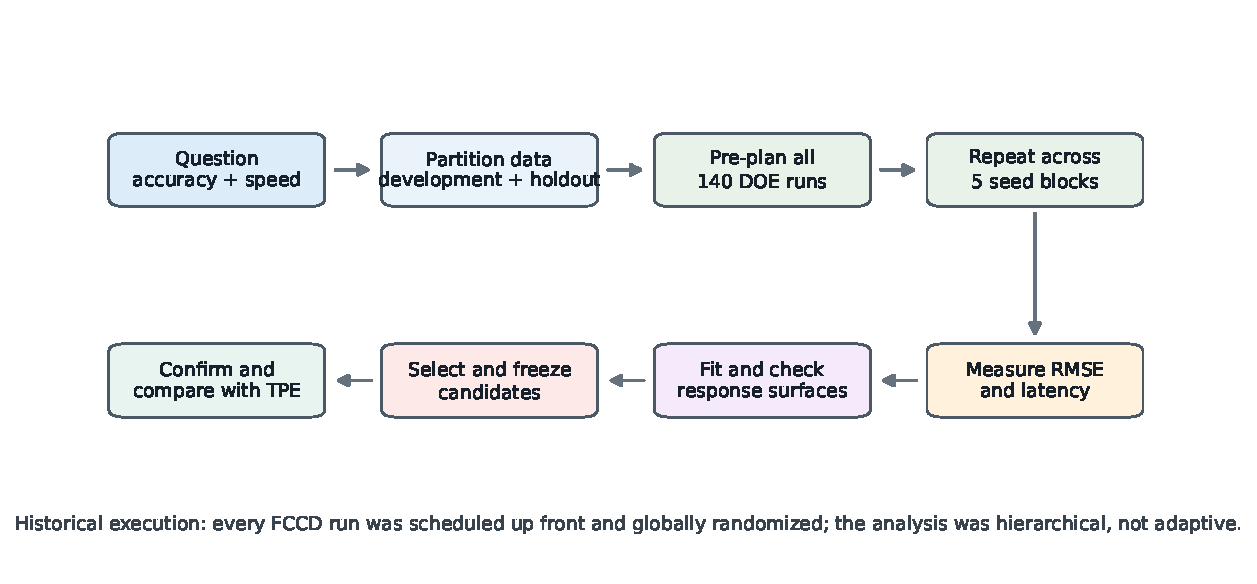
\includegraphics[width=\textwidth]{figures/phase_a_workflow.pdf}
\caption{Structure of the housing experiment: a planned design, hierarchical response analysis, compromise selection and independent confirmation.}\end{figure}
\subsection{Performance measures and multi-objective selection}
For housing regression, \term{root mean squared error (RMSE)} measures prediction error, giving extra weight to large errors. Smaller is better. For sentiment classification, \term{macro F1} averages the F1 scores of the sentiment classes, giving each class equal weight. Larger is better. The optimization response in Phase B is one minus macro F1, so smaller is better. \term{Log loss} additionally checks the quality of predicted probabilities and penalizes confident mistakes.
\term{Latency} measures the time needed for a trained model to predict an observation. Lower latency is preferable, but the exact operation matters: constructing an input wrapper, transforming raw text and predicting an already-vectorized document are different tasks. A latency value is meaningful only with its measurement protocol.
When no configuration is best on both accuracy and latency, we examine the \term{Pareto front}: configurations for which no tested alternative improves one objective without worsening the other. \term{Hypervolume} summarizes the area dominated by that front relative to a declared reference point. Larger hypervolume is preferable under the same objectives and reference. Hypervolumes from different tasks or reference points cannot be compared directly.
\section{Phase A: experimental design}
\subsection{A planned design with stochastic nuisance blocks}
The historical design contains \m{ADesign} fitted evaluations across \m{ABlocks} data-split blocks. It studies learning rate, maximum depth, row subsampling and leaf-weight regularization. A globally randomized, preplanned face-centered CCD supplies the observations. The factorial and augmented analyses are hierarchical analyses of that completed design; they are not evidence that an early result adaptively determined whether the later points were run.
California Housing~\cite{housing} is divided into \m{ASplittrain}\% training, \m{ASplitval}\% validation and \m{ASplittest}\% test data, with \m{ACapacity} boosting trees per model. The model predicts median house values; RMSE retains the dataset's target scale. The split is randomized, so this study does not test transfer to geographically separated regions. Early exploratory work exposed test outcomes; later access restrictions cannot undo that exposure.
The block represents the seeded data partition, not a geographic region. Repeated center evaluations vary the model's stochastic seed while preserving the relevant split. This allows local algorithmic variation to be distinguished from larger changes between configurations and partitions, though those sources should not be interpreted as independent draws from all possible datasets.
\begin{table}[!htbp]\centering\begin{tabular}{lrr}
\toprule
Factor & Phase A range & Phase B range \\
\midrule
Learning rate & [\m{AFactorALow}, \m{AFactorAHigh}] & [\m{BFactorALow}, \m{BFactorAHigh}] \\
Tree depth & [\m{AFactorBLow}, \m{AFactorBHigh}] & [\m{BFactorBLow}, \m{BFactorBHigh}] \\
Row subsampling & [\m{AFactorCLow}, \m{AFactorCHigh}] & [\m{BFactorCLow}, \m{BFactorCHigh}] \\
Regularization & [\m{AFactorDLow}, \m{AFactorDHigh}] & [\m{BFactorDLow}, \m{BFactorDHigh}] \\
\bottomrule
\end{tabular}

\caption{Hyperparameter ranges in the two phases. Learning rate uses logarithmic coding in Phase A and linear coding in Phase B; regularization uses logarithmic coding in both.}\end{table}
\begin{figure}[!htbp]\centering
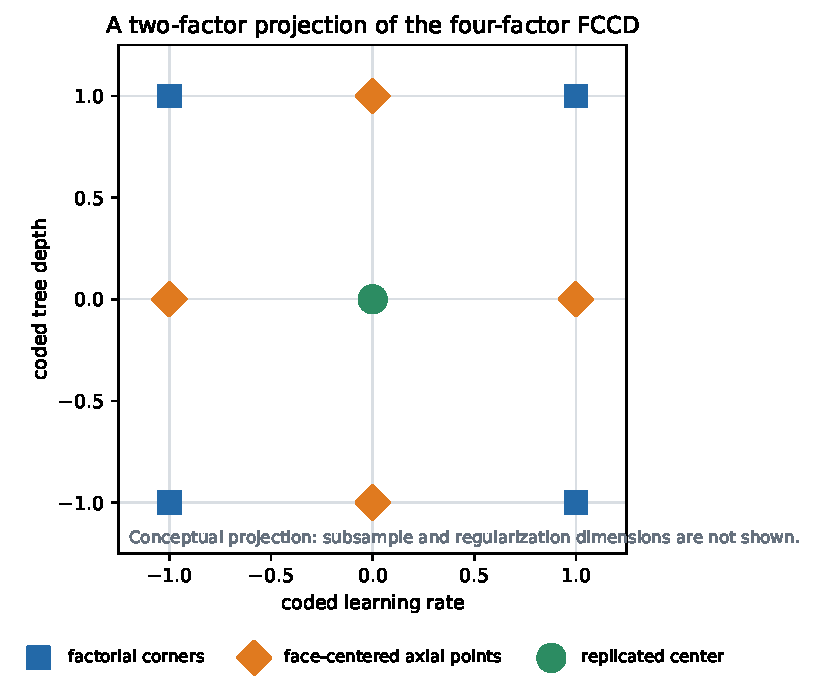
\includegraphics[width=0.48\textwidth]{figures/phase_a_design.pdf}\hfill
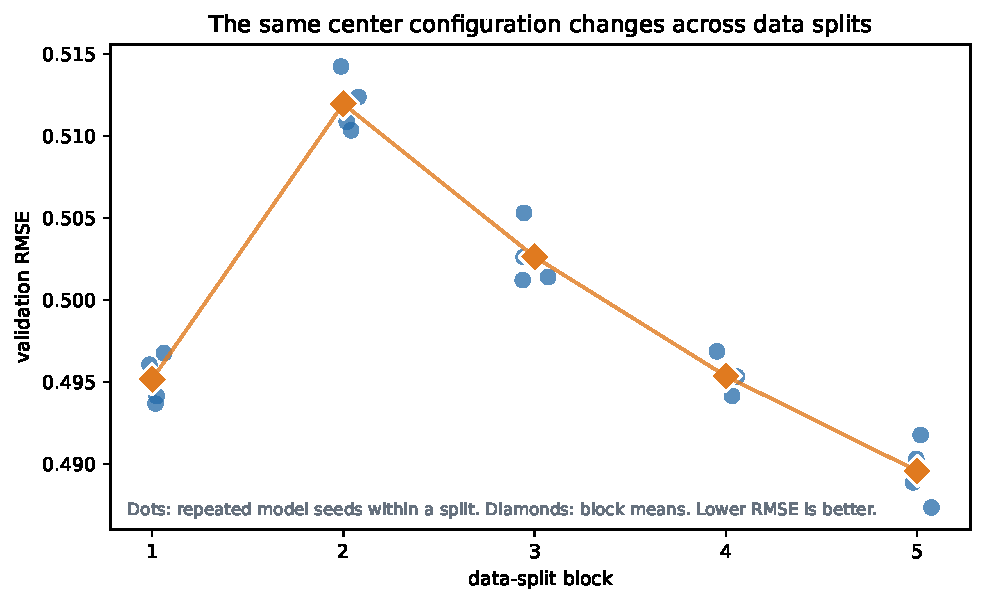
\includegraphics[width=0.48\textwidth]{figures/phase_a_blocking.pdf}
\caption{Phase A design and blocking. Left: a projection of the central composite design onto learning rate and depth. Right: center-point outcomes across data-split blocks show why partition effects must be distinguished from hyperparameter effects.}\end{figure}
\subsection{Screening, response fitting and selection}
The first analysis asks whether a flat first-order model is adequate. A strong curvature contrast leads to examining a quadratic response model. The model contains main effects, pairwise interactions and squared terms, together with block effects. \term{ANOVA} partitions modeled variation and supplies model-conditional tests for these terms.
We use the fitted error and latency surfaces to explore candidate configurations. An accuracy-focused choice minimizes predicted error; the compromise uses Derringer--Suich desirability~\cite{desirability}:
\begin{equation}\label{eq:desirability}
d_m(y)=\begin{cases}1,&y\le L_m,\\ \left(\dfrac{U_m-y}{U_m-L_m}\right)^{s_m},&L_m<y<U_m,\\0,&y\ge U_m,\end{cases}
\quad D(\mathbf{x})=\left[\prod_m d_m(\widehat Y_m(\mathbf{x}))^{w_m}\right]^{1/\sum_m w_m}.
\end{equation}
The recorded RMSE limits are \m{DesirabilityErrorLow} and \m{DesirabilityErrorHigh}; latency limits are \m{DesirabilityLatencyLow} and \m{DesirabilityLatencyHigh}\,$\mu$s. The shape exponents and response weights equal \m{DesirabilityExponent}. These are preference settings, not estimated physical constants. Selected candidates receive separate confirmation evaluations.
The subsequent repeated benchmark compares DOE selections with tree-structured Parzen estimator (TPE) search~\cite{tpe} and random search~\cite{randomsearch}. TPE updates probabilistic models of promising and less promising trials to propose new settings. Each method receives the same fit budget, but DOE distributes fits across planned coordinates and data splits while the black-box searches explore configurations on a fixed development split. It is separate from the historical design and confirmation stage.
\section{Phase A: results and limitations}
\subsection{Useful structure, but not a perfect surface}
The factorial-to-center curvature statistic is \m{ACurvature}. The response clearly departs from a flat plane over the tested range. The block-variance analysis reports an RMSE intraclass correlation of \m{AIcc}\%. This supports treating data partition as a meaningful nuisance condition rather than ignoring it.
However, strong global structure is not the same as local predictive accuracy. The RMSE surface has a lack-of-fit statistic of \m{ALof}. A smooth quadratic equation captures major trends yet misses some systematic response behavior. The curvature contrast uses center-point pure error, whereas the stored lack-of-fit analysis has a different replicate-error decomposition. These denominators must not be conflated, and neither automatically represents uncertainty over all future datasets.
The lowest learning rate, \m{ALowRate}, occurs in \m{ALowCount} of \m{ADesign} runs (\m{ALowPct}\%); that allocation follows the CCD geometry. The issue is whether the chosen range learns adequately under the fixed tree budget. New post-hoc diagnostics give lack-of-fit $F=\m{PostLogLof}$ after log-transforming RMSE and $F=\m{PostRestrictedLof}$ after excluding that low-rate face. The restricted fit has $R^2=\m{PostRestrictedRtwo}$ but rank \m{PostRestrictedRank} of \m{PostRestrictedColumns}: its remaining learning-rate linear and squared terms are aliased. Thus neither transformation nor exclusion establishes an adequate quadratic model or localizes all misspecification to the low-rate face.
Figure~\ref{fig:adiagnostics} plots residuals, the differences between observed and fitted responses, on the original and log scales. Persistent structure and departures from the normal reference line caution against treating model-based intervals as fully calibrated.
\begin{figure}[!htbp]\centering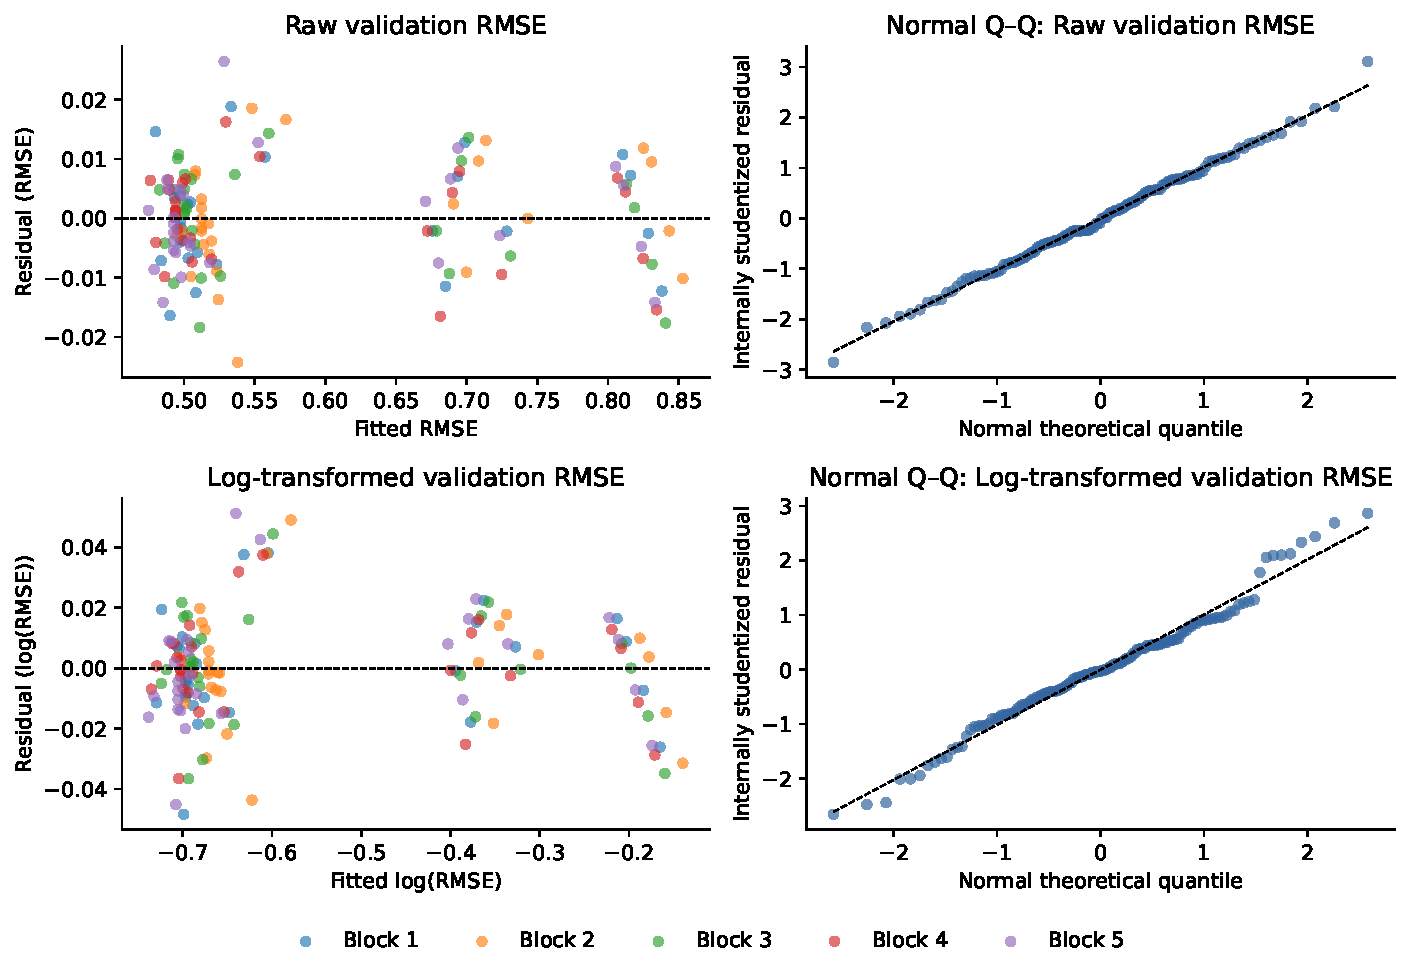
\includegraphics[width=\textwidth]{figures/phase_a_diagnostics.pdf}
\caption{Post-hoc Phase A diagnostics of the quadratic model with fixed block effects. Left: residuals versus fitted values, colored by data-partition block. Right: normal quantile plots of internally studentized residuals. Log transformation does not remove the model-adequacy concern.}\label{fig:adiagnostics}\end{figure}
\begin{figure}[!htbp]\centering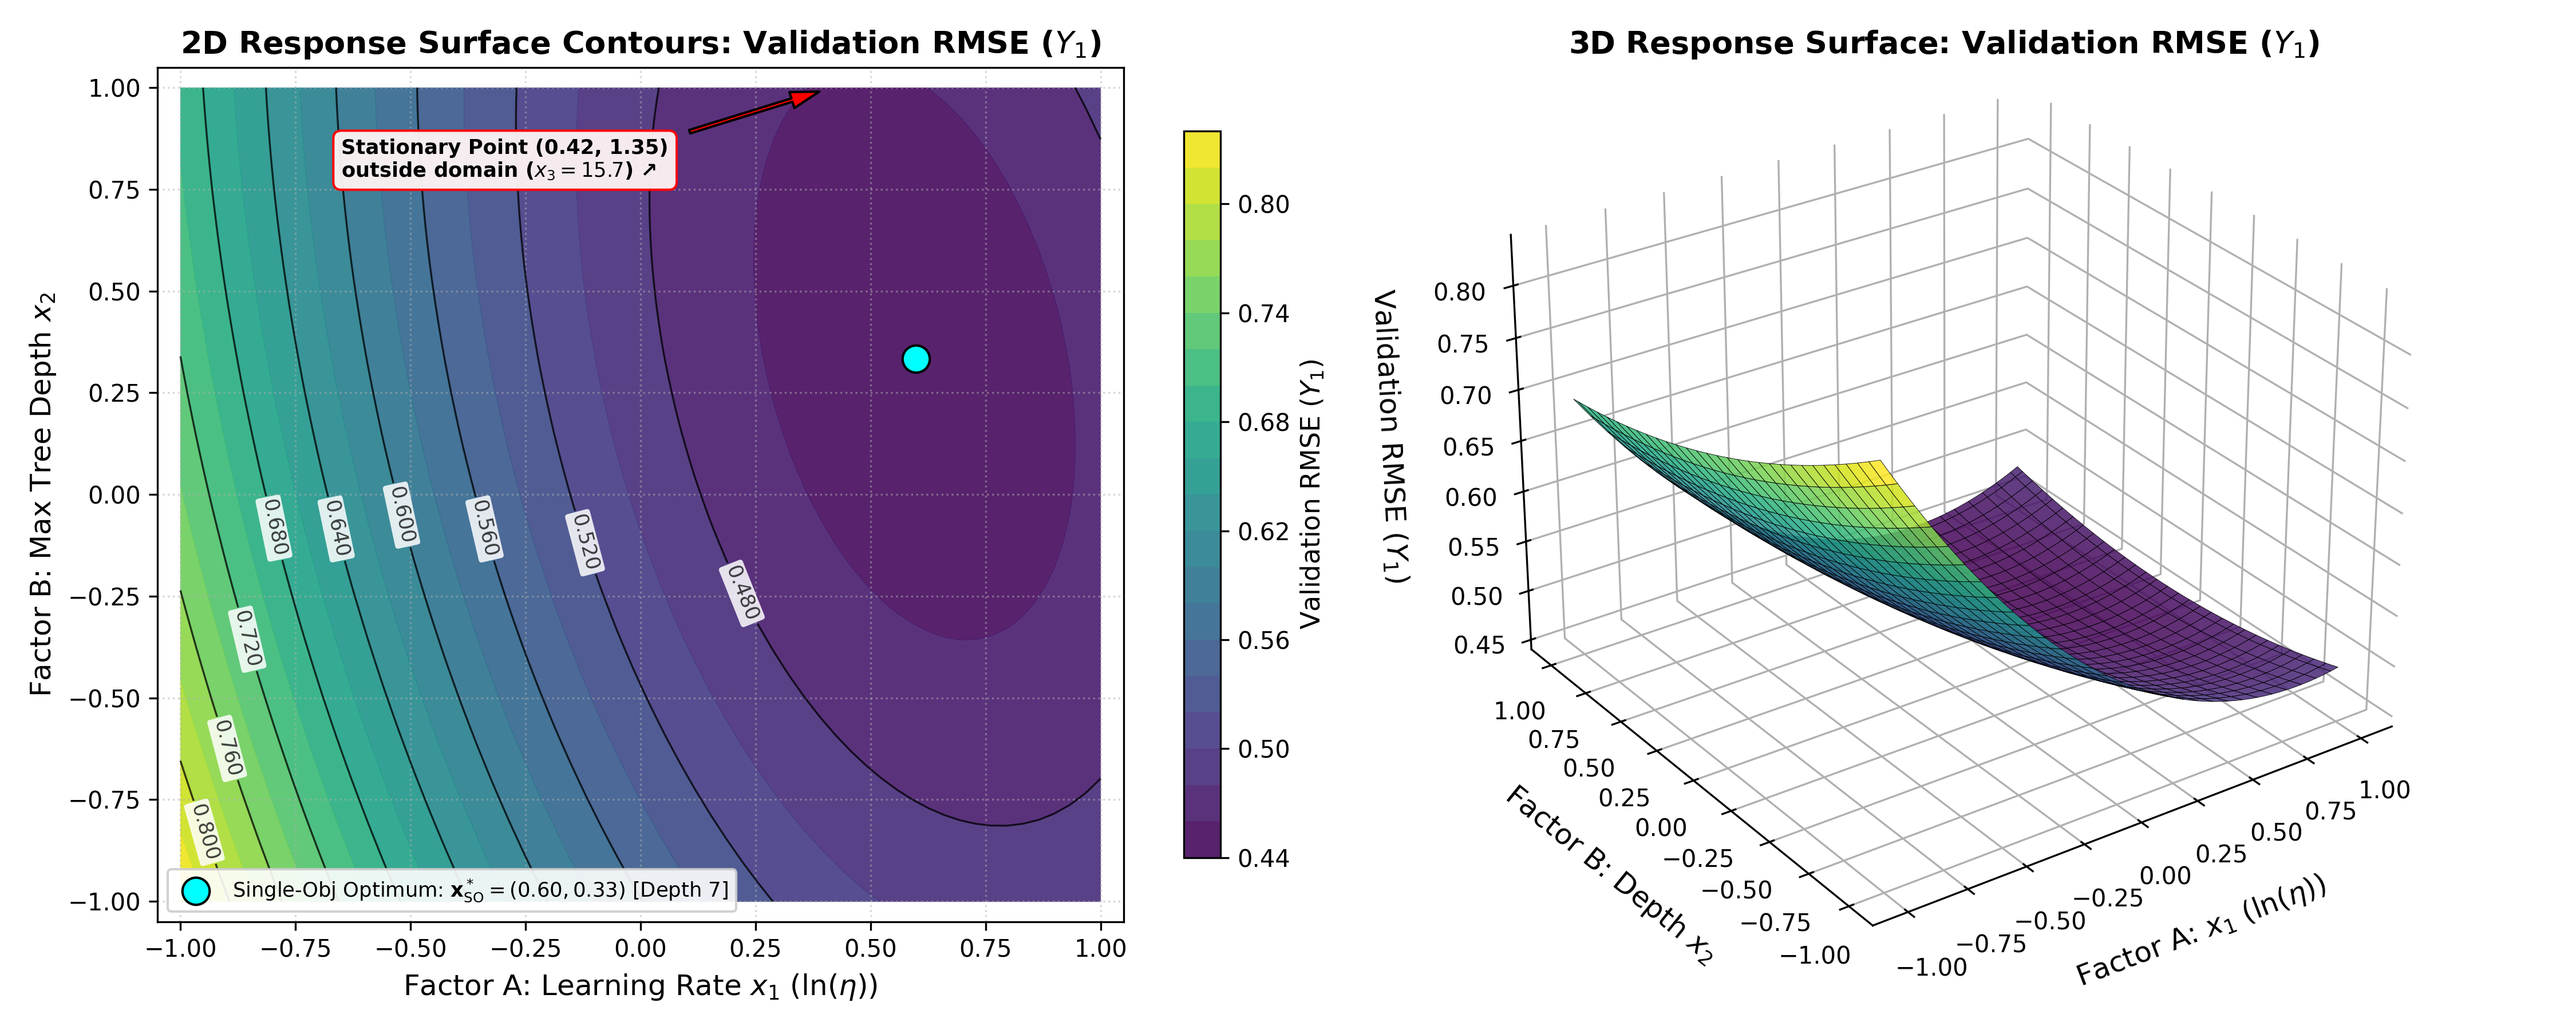
\includegraphics[width=\textwidth]{figures/phase_a_error_surface.png}
\caption{Phase A fitted validation-error surface across coded learning rate and tree depth. Contours and the three-dimensional view show broad curvature, while the out-of-domain stationary point illustrates the danger of extrapolating a fitted optimum.}\end{figure}
\begin{figure}[!htbp]\centering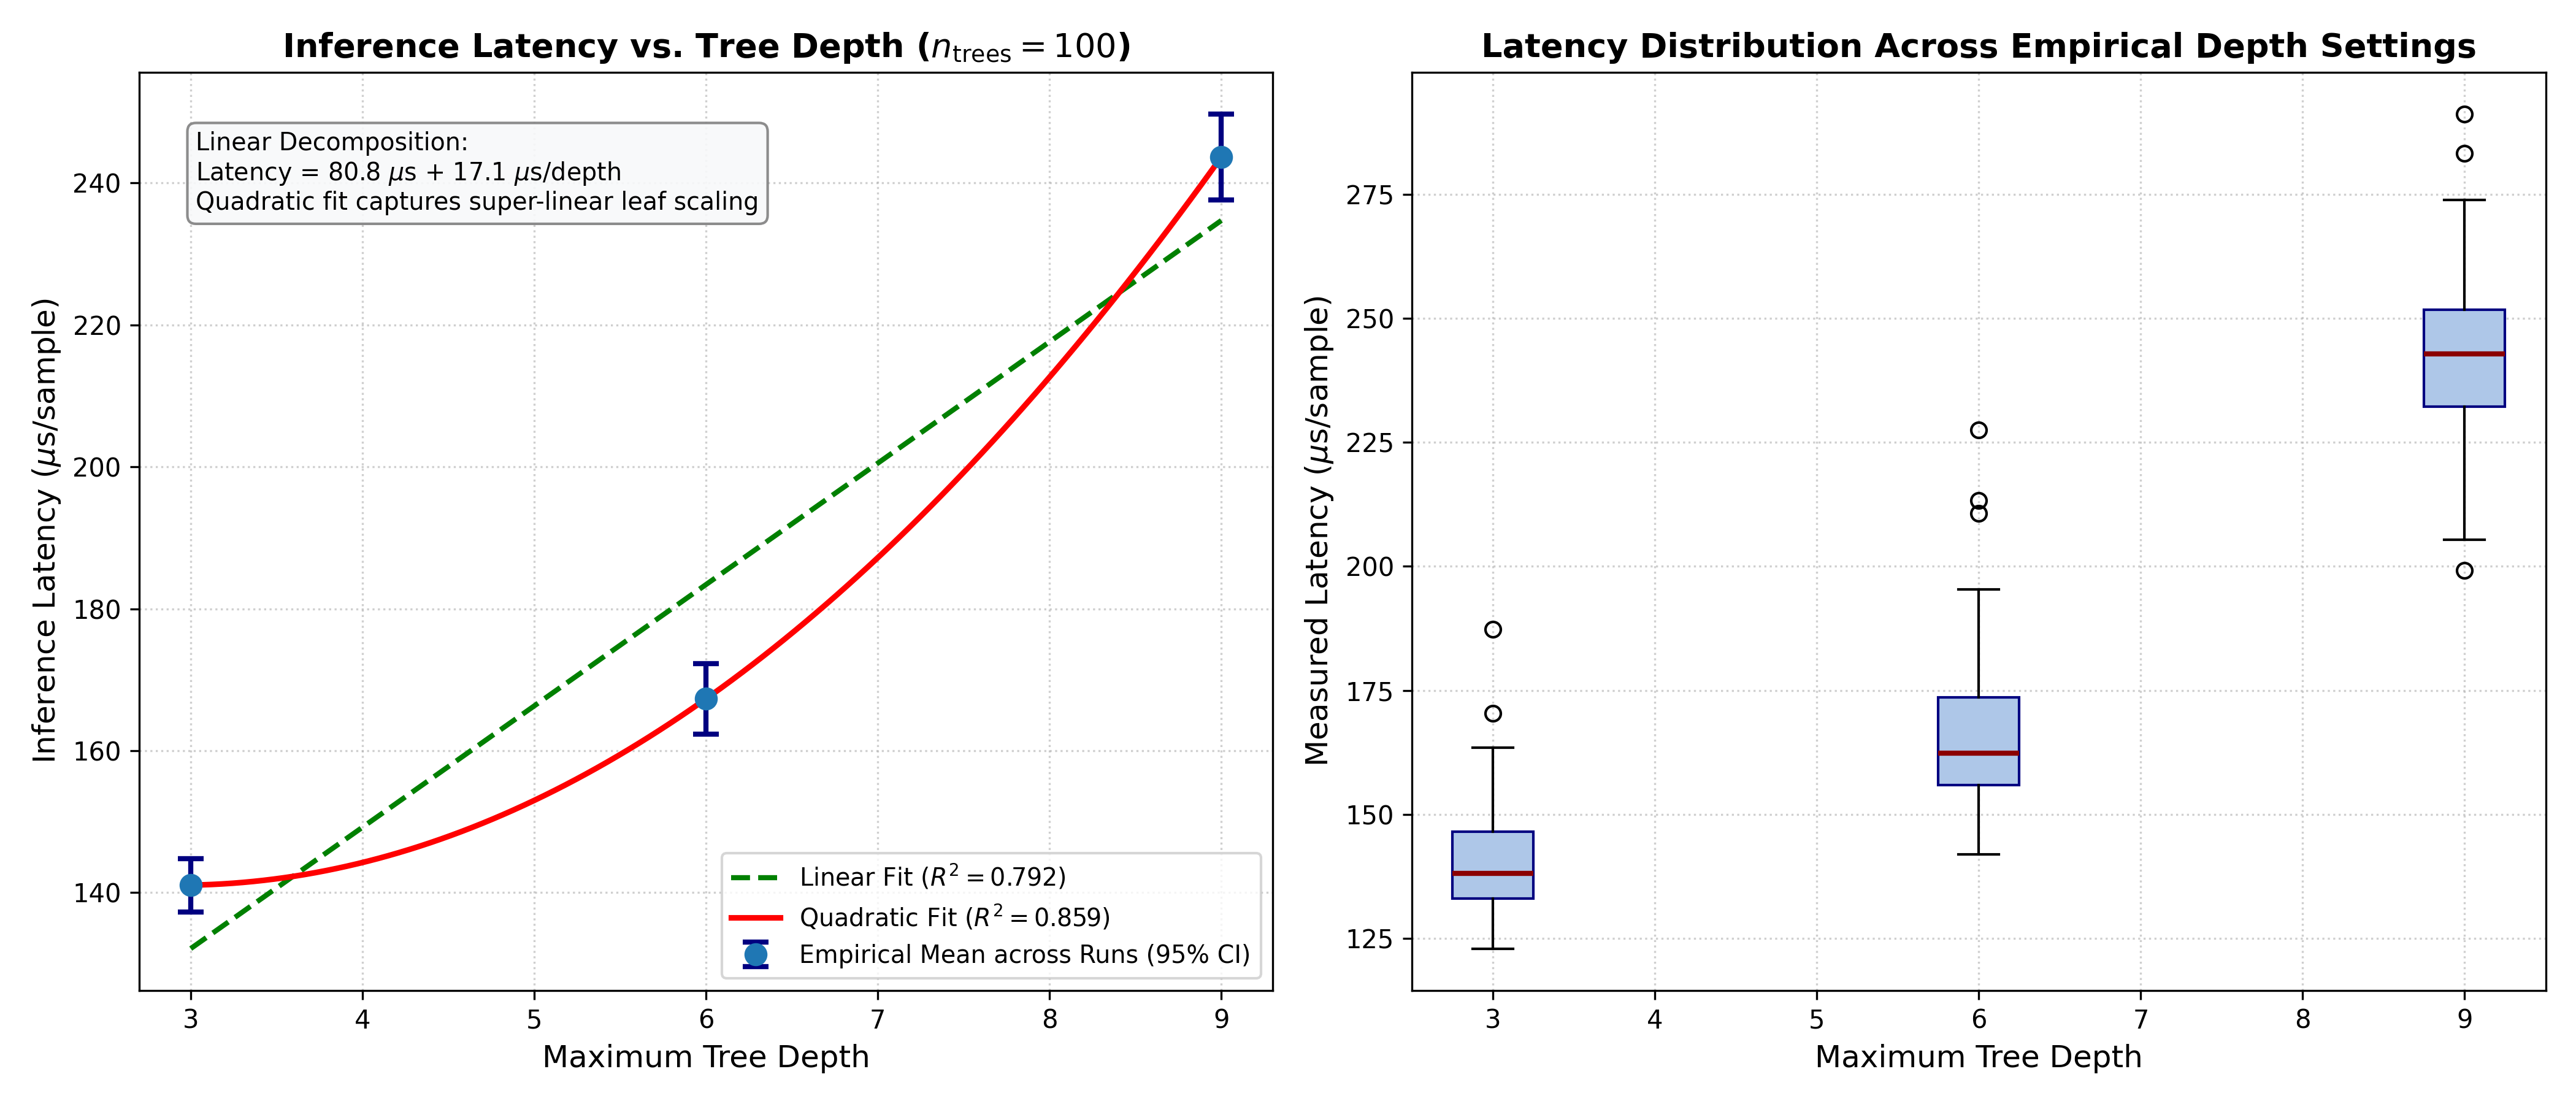
\includegraphics[width=\textwidth]{figures/phase_a_latency.png}
\caption{Phase A CPU prediction latency across tree depths. Linear and quadratic fits summarize the change in cost; distributions show variation among measured runs.}\end{figure}
\subsection{Confirmation revealed boundary optimism}
Table~\ref{tab:aconfirm} compares the surface with confirmation on new data-split seeds, disjoint from the design's split seeds but using the same housing dataset. The compromise candidate's observed validation RMSE falls within its interval. The accuracy-focused candidate lies above its upper bound; its observed-minus-predicted gap is \m{AAccuracyBias} RMSE. These are working-model intervals from a demonstrably imperfect surface; the gap combines model inadequacy and split variation rather than identifying either cause alone.
\begin{table}[!htbp]\centering\begin{tabular}{lrrr}
\toprule
Candidate & Predicted & Interval & Observed \\
\midrule
Balanced & \m{ABalancedPred} & $[\m{ABalancedLower}, \m{ABalancedUpper}]$ & \m{ABalancedObs} \\
Accuracy & \m{AAccuracyPred} & $[\m{AAccuracyLower}, \m{AAccuracyUpper}]$ & \m{AAccuracyObs} \\
\bottomrule
\end{tabular}

\caption{Phase A validation-RMSE confirmation. Model-based \m{AIntervalLevel}\% prediction intervals target the mean of \m{AConfirmationCount} confirmation runs per candidate; the observed column is that mean. The intervals do not cover every possible future dataset outcome.}\label{tab:aconfirm}\end{table}
\begin{figure}[!htbp]\centering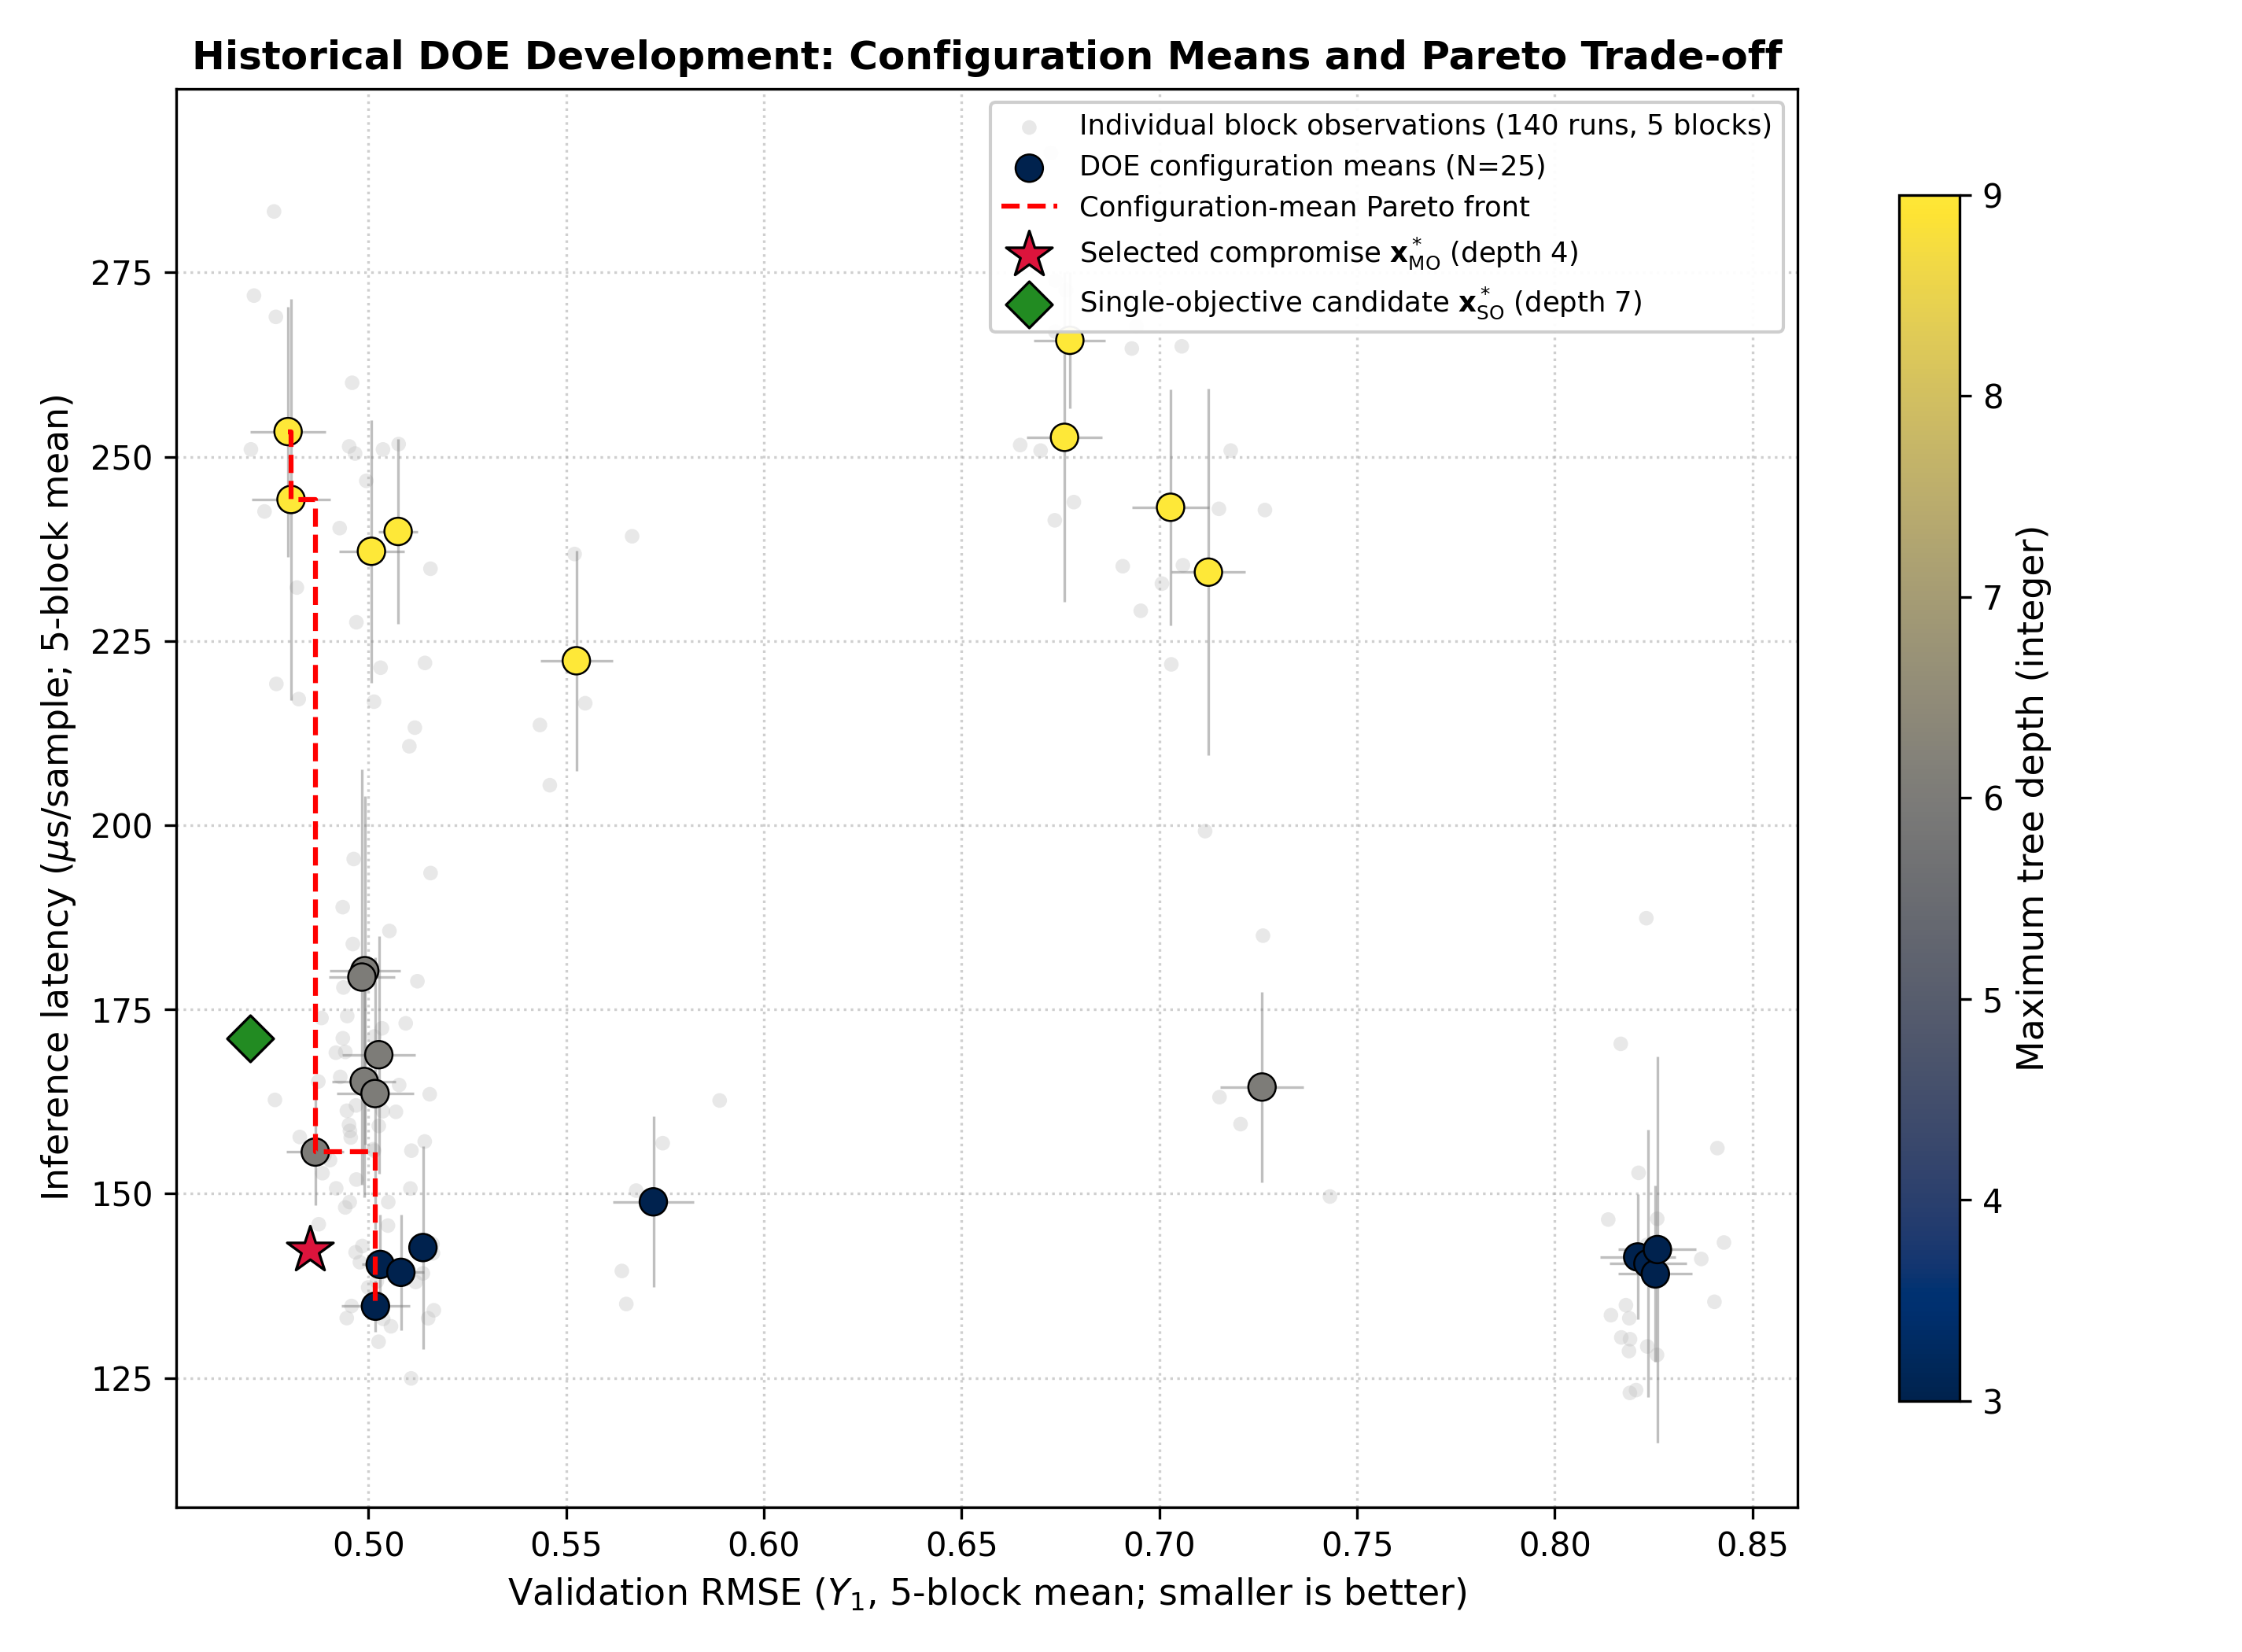
\includegraphics[width=\textwidth]{figures/phase_a_tradeoff.png}
\caption{Phase A accuracy--speed trade-off among the initial design configurations. Configuration means and between-block uncertainty distinguish the compromise candidate from the accuracy-focused candidate.}\end{figure}
\subsection{Optimizer comparison and latency feasibility}
Table~\ref{tab:abench} summarizes \m{ARepeats} searches per method, with \m{AEvaluationCount} retraining evaluations per selection. Its error SD describes variability between search-level mean test errors. The displayed zero for DOE accuracy reflects repeated selection of the same configuration and the same evaluation seeds; it does not mean error-free prediction or zero retraining variability.
\begin{table}[!htbp]\centering\small\resizebox{\textwidth}{!}{\begin{tabular}{lrrrr}
\toprule
Method & Test RMSE & Between-search SD & Within-selection SD & CPU latency ($\mu$s) \\
\midrule
Repeated DOE compromise & \m{ABenchAError} & \m{ABenchASd} & \m{PostWithinA} & \m{ABenchALatency} \\
Repeated DOE accuracy & \m{ABenchBError} & \m{ABenchBSd} & \m{PostWithinB} & \m{ABenchBLatency} \\
MO-TPE & \m{ABenchCError} & \m{ABenchCSd} & \m{PostWithinC} & \m{ABenchCLatency} \\
Constrained TPE & \m{ABenchDError} & \m{ABenchDSd} & \m{PostWithinD} & \m{ABenchDLatency} \\
Accuracy-focused TPE & \m{ABenchEError} & \m{ABenchESd} & \m{PostWithinE} & \m{ABenchELatency} \\
Random search & \m{ABenchFError} & \m{ABenchFSd} & \m{PostWithinF} & \m{ABenchFLatency} \\
\bottomrule
\end{tabular}
}
\caption{Phase A selected-model results. Between-search SD is the SD of selection-level mean test RMSE; within-selection SD is the mean of the SDs across retraining seeds. RMSE is lower-is-better and CPU latency is in microseconds. Identical repeated selections are not independent discoveries of an optimum.}\label{tab:abench}\end{table}
The accuracy-focused TPE strategy attains lower observed error at a greater latency cost than the compromise strategies. This is evidence of a trade-off, not a universal winner. DOE invests observations in structured comparisons and replication; adaptive optimizers spend more on distinct proposed configurations.
Latency also exposes a measurement problem. At the predeclared \m{ACap}\,$\mu$s threshold, Constrained TPE appears feasible in \m{ASearchFeasible} of \m{ARepeats} searches but only \m{AVerifiedFeasible} selections remain feasible under benchmark verification. The short online timing and longer final measurement differ in cost and precision. Selection near a noisy boundary can amplify their disagreement. The data do not establish one unique causal explanation for the discrepancy.
\begin{figure}[!htbp]\centering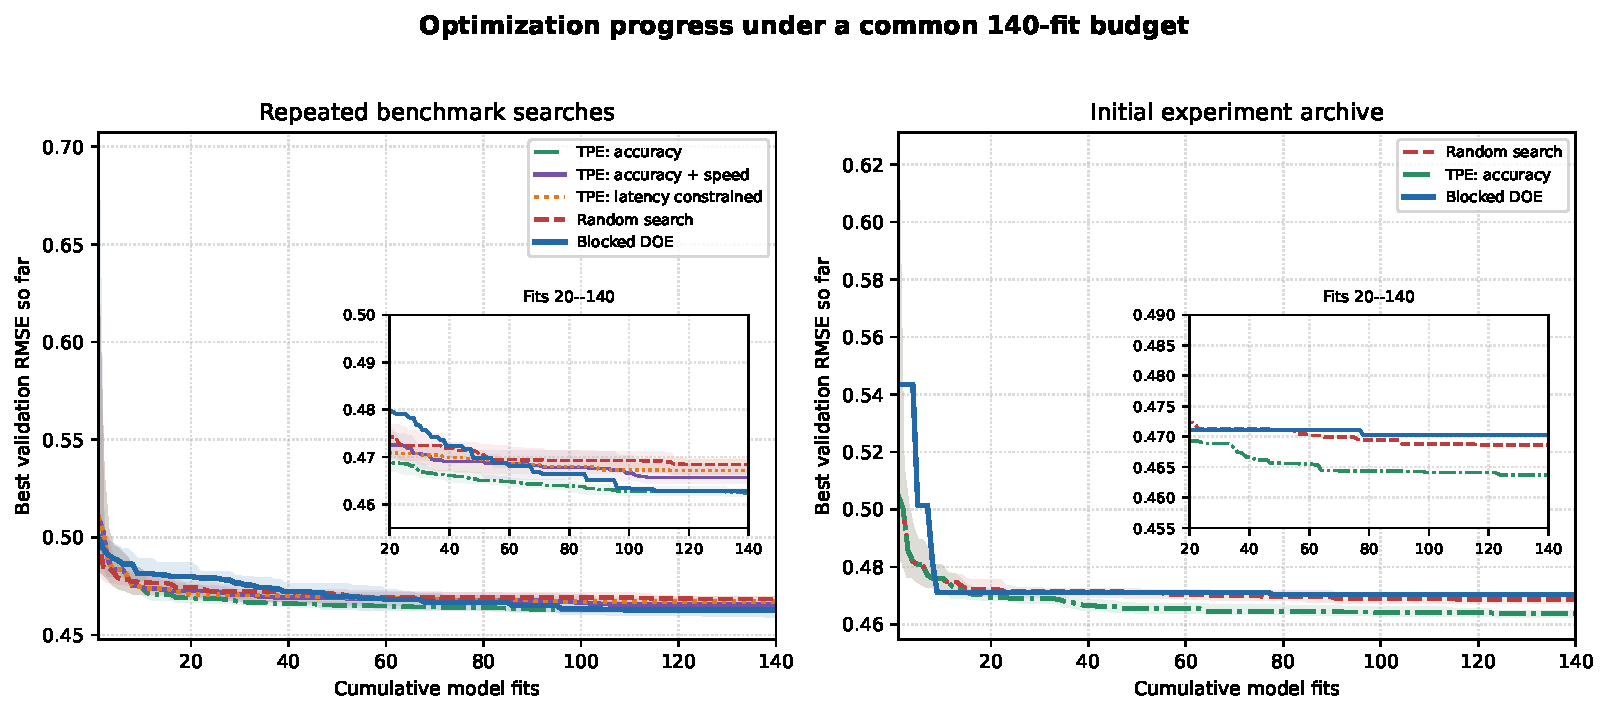
\includegraphics[width=\textwidth]{figures/phase_a_efficiency.pdf}
\caption{Phase A search trajectories under equal fit budgets. Curves summarize the recorded validation histories; DOE uses multiple validation blocks, so these are descriptive efficiency curves rather than a common-estimand proof of optimizer superiority.}\end{figure}
\begin{figure}[!htbp]\centering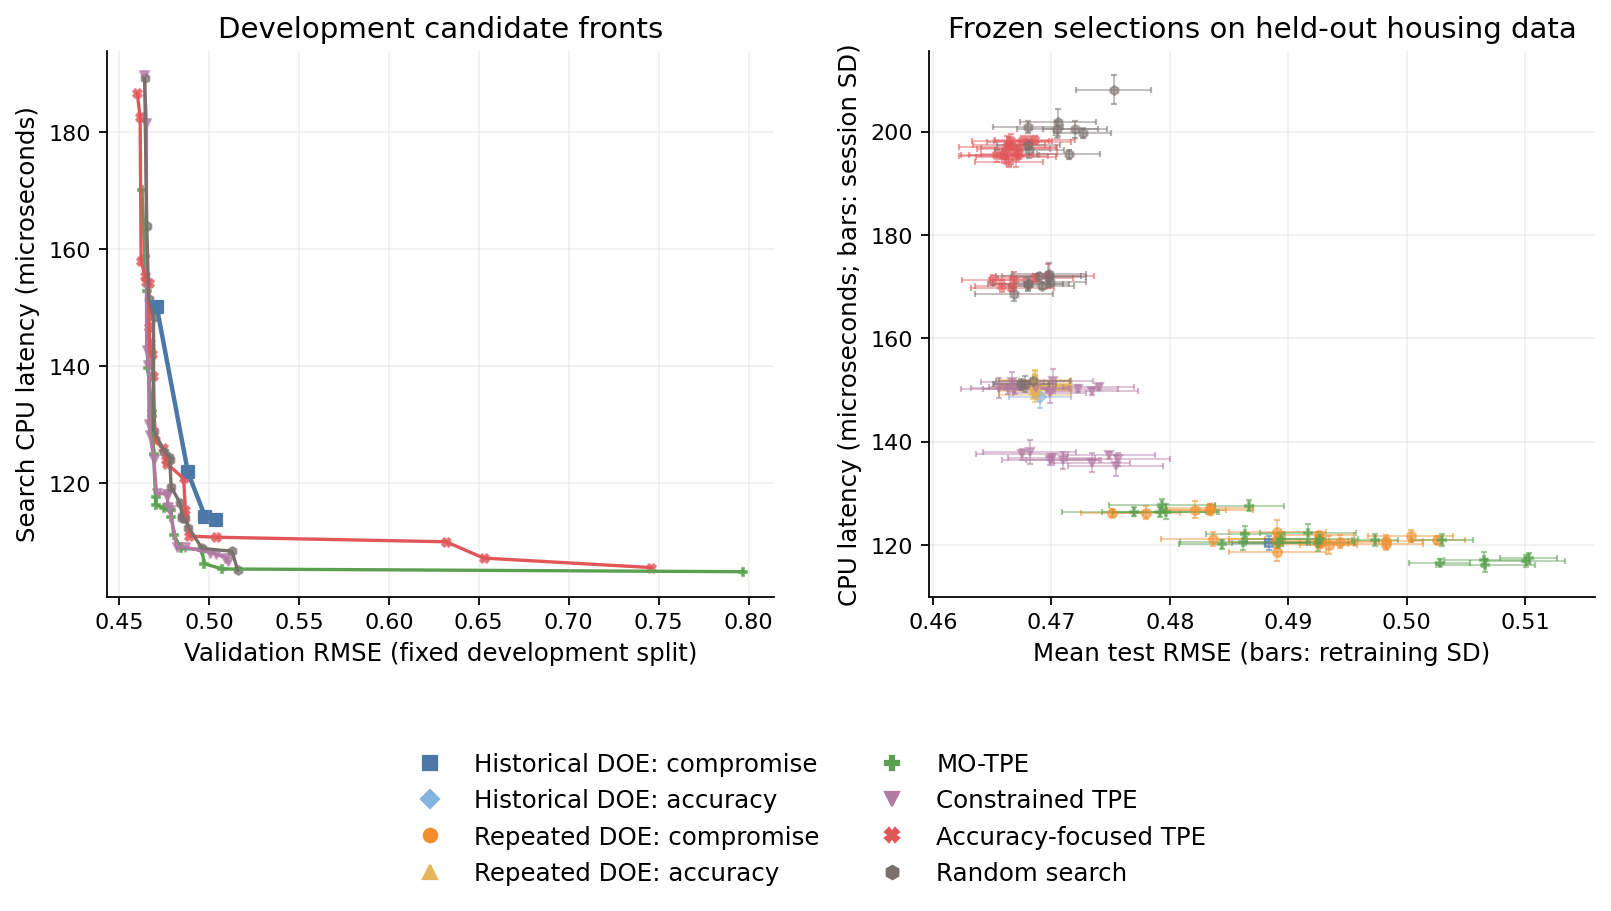
\includegraphics[width=\textwidth]{figures/phase_a_pareto.png}
\caption{Phase A Pareto comparisons. Left: pooled fixed-split development trial fronts provide context. Right: each point is a frozen selection; RMSE bars show within-selection retraining SD and latency bars show measurement-session SD. Development and test panels describe separate stages.}\end{figure}
\section{Motivation and research question for Phase B}
Phase A establishes that DOE can explain substantial structure and select useful compromise models. It simultaneously identifies reasons to change the next experiment. The learning-rate domain needs development-only calibration; final timing must measure the same operation as search; test history must be stated honestly; and surrogate predictions need checks at genuinely unused hyperparameter coordinates.
The next scientific question is therefore:
\begin{quote}\textbf{How does a small GP-guided extension change a static CCD, and how do sampling geometry and response-model choice affect confirmation and diagnostic explanations?}\end{quote}
Moving to sentiment classification gives a sparse feature space and a second interpretation problem: explaining how selected word-feature changes affect an individual classifier prediction.
Phase B has several connected objectives: compare ANOVA and SHAP for the same response; predict unseen configurations; test a modest adaptive extension against static CCD; benchmark both against TPE; and evaluate local word-response explanations. These objectives must remain distinguishable. Good classifier accuracy does not automatically establish good explanations, and agreement between explanations does not establish accurate response prediction.
\begin{figure}[!htbp]\centering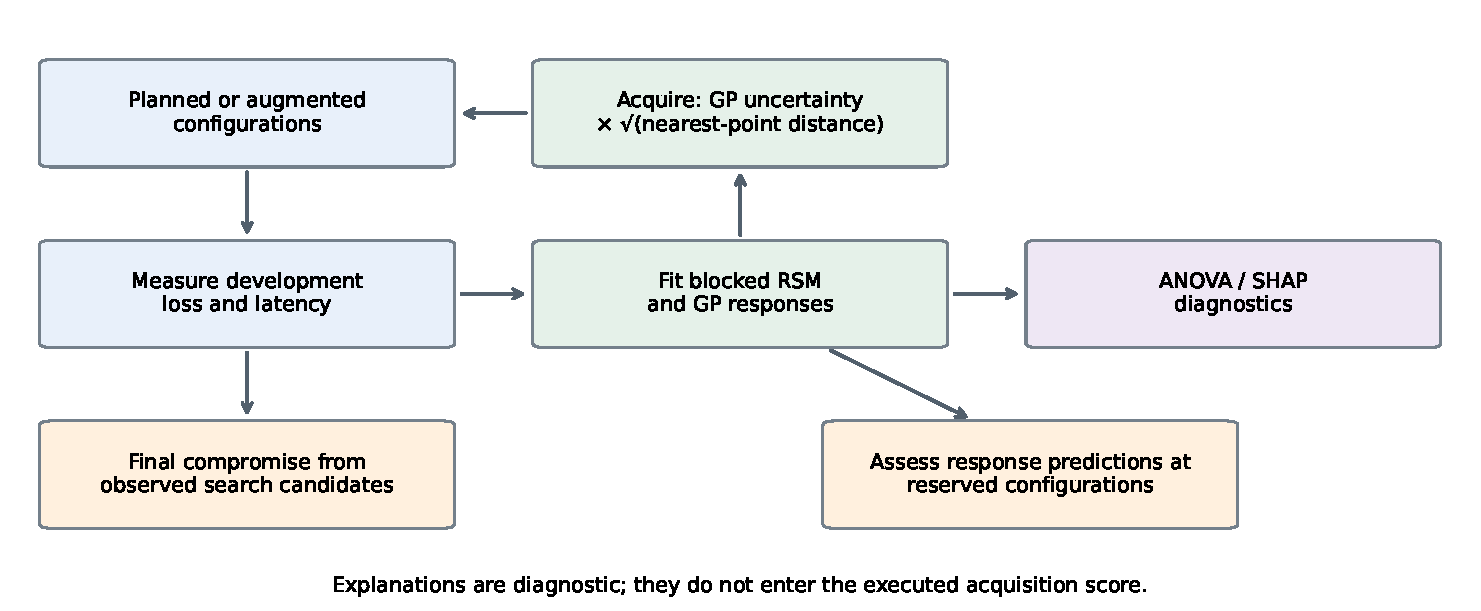
\includegraphics[width=\textwidth]{figures/sequential_design.pdf}
\caption{Executed sequential design. GP uncertainty and distance guide new evaluations; ANOVA and SHAP form a diagnostic branch. Final selection uses observed development responses. Reserved responses assess surrogate predictions, and are excluded from fitting and acquisition.}\end{figure}
\section{Phase B: experimental methodology}
\subsection{Data, preprocessing and evaluation}
The IMDb movie-review dataset~\cite{imdb} supplies \m{BDev} development documents and \m{BTest} test documents after HTML removal, whitespace normalization and exact-text deduplication. Official test copies are retained when duplicates span the two partitions. Term frequency--inverse document frequency (TF-IDF) converts each document into a sparse vector of word and word-pair weights, using at most \m{BVocab} features and sublinear term frequency. Vocabulary and weights are fitted within each training fold, so validation text does not determine that fold's representation.
The development pool is partitioned into \m{BBlocks} stratified folds. Every method evaluates a proposed configuration on the same folds and receives the mean response across them. The folds are useful shared nuisance conditions, but their training observations overlap. Different optimizer seeds on those folds do not create independently sampled datasets.
All selected configurations are fixed before final test evaluation. Because the test partition has prior exposure, these scores are not fully independent external confirmation. This limits the generalization claim.
\subsection{Calibration and computational setting}
The lower learning-rate boundary is now \m{BRateLow}. Development calibration compares tree budgets before fixing the main study's capacity. At the low rate, observed calibration macro F1 changes from \m{CalSmall} at \m{CalSmallTrees} trees to \m{CalLarge} at \m{BTrees} trees. The capacity rule chooses the smallest tested budget whose low-rate F1 is within \m{BCalTolerance} of the largest tested budget, selecting \m{BTrees} trees. This reduces the low-capacity problem within the tested grid; it does not prove that larger models cannot improve.
Models are trained on an \AcceleratorName{} accelerator. Prediction latency and local word-response probabilities are measured on CPU. This separates training acceleration from the inference operation being evaluated.
\begin{table}[!htbp]\centering\small\begin{tabular}{lrrr}
\toprule
Trees & Learning rate & Validation macro F1 & CPU latency ($\mu$s) \\
\midrule
\m{CalibrationATrees} & \m{CalibrationARate} & \m{CalibrationAFone} & \m{CalibrationALatency} \\
\m{CalibrationBTrees} & \m{CalibrationBRate} & \m{CalibrationBFone} & \m{CalibrationBLatency} \\
\m{CalibrationCTrees} & \m{CalibrationCRate} & \m{CalibrationCFone} & \m{CalibrationCLatency} \\
\m{CalibrationDTrees} & \m{CalibrationDRate} & \m{CalibrationDFone} & \m{CalibrationDLatency} \\
\m{CalibrationETrees} & \m{CalibrationERate} & \m{CalibrationEFone} & \m{CalibrationELatency} \\
\m{CalibrationFTrees} & \m{CalibrationFRate} & \m{CalibrationFFone} & \m{CalibrationFLatency} \\
\bottomrule
\end{tabular}

\caption{Phase B development calibration. Tree count is selected before the main study; accuracy and timing change with capacity. The timings are calibration observations, not final-model serving guarantees.}\end{table}
\subsection{A fair comparison with a small adaptive extension}
Static CCD, sequential CCD and MO-TPE each receive \m{BFitsPerSearch} actual XGBoost fits per search repeat. The comparison uses \m{BRepeats} repeats. A proposed coordinate is evaluated on every development fold, so model-fit count must not be confused with unique configuration count.
The budget supplies \m{PostProposalBudget} complete-fold configuration evaluations per search; CCD center replications reuse coordinates. This is a small optimization budget for assessing an adaptive sampler's startup and subsequent learning.
Static CCD retains its center replication. Sequential CCD reallocates center fits to \m{PostAdaptiveCoordinates} adaptive coordinates per search repeat. Its Gaussian processes (GPs) use scaled Mat\'ern covariance with fitted factor-specific length scales and white noise, following the computer-experiment surrogate approach~\cite{sacks,santner}. The executed acquisition is
\begin{equation}\label{eq:acquisition}
a(\mathbf{x})=\sqrt{\left(\frac{\sigma_\ell(\mathbf{x})}{r_\ell}\right)^2+\left(\frac{\sigma_t(\mathbf{x})}{r_t}\right)^2}\;\sqrt{d_{\min}(\mathbf{x})},\qquad
d_{\min}(\mathbf{x})=\min_{\mathbf{z}\in\mathcal D}\|\mathbf{x}-\mathbf{z}\|_2.
\end{equation}
The reference coordinates $r_\ell,r_t$ normalize objective uncertainty. $\mathcal D$ includes existing and reserved coordinates, and candidates too close to that set are rejected. Surrogates are refitted after augmentation. GP uncertainty therefore makes an acquisition decision, but neither SHAP scores nor a predicted response optimum determine the final selected classifier.
MO-TPE~\cite{motpe}, implemented with Optuna~\cite{optuna}, proposes configurations from the same domain and receives the same block-mean loss and latency responses. All methods select an observed compromise by maximizing
\begin{equation}\label{eq:selection}
S(\ell,t)=\max(0,r_\ell-\ell)\max(0,r_t-t).
\end{equation}
This rectangle rule is a preference over measured configurations; it is distinct from the hypervolume of the full observed front and imposes no hard latency constraint.
The complete Phase B experiment contains \m{BSearch} search fits, \m{BConfirmationFits} confirmation fits and \m{BFinalFits} final refits, plus the local explanation model: \m{BTotal} new model fits in total. Total runtime is \m{BHours} hours; this excludes the preceding calibration and is not a measured CPU-versus-GPU speedup.
\begin{table}[!htbp]\centering\begin{tabular}{lrrr}
\toprule
Method & Initial/search fits & Adaptive fits & Total per search \\
\midrule
Static CCD & \m{BudgetstaticdoeInitial} & \m{BudgetstaticdoeInfill} & \m{BudgetstaticdoeTotal} \\
Sequential CCD & \m{BudgetdoeInitial} & \m{BudgetdoeInfill} & \m{BudgetdoeTotal} \\
MO-TPE & \m{BudgettpeInitial} & \m{BudgettpeInfill} & \m{BudgettpeTotal} \\
\bottomrule
\end{tabular}

\caption{Phase B fit allocation per method and search repeat, including all development folds. Sequential CCD reallocates center replication to adaptive points while preserving the total budget. TPE's proposals are reported as search fits.}\end{table}
\subsection{The timing protocol and what the threshold means}
The common measurement operation uses \m{BWarmups} warmups followed by \m{BCalls} timed predictions per interface, with CPU affinity and single-thread prediction recorded. The primary operation includes fresh DMatrix construction plus prediction of one already-vectorized document; \texttt{inplace\_predict} is recorded separately. Raw-text TF-IDF transformation is excluded.
The measurement uses the first validation row in each fold. It supports an input-specific microbenchmark, not a latency distribution over representative documents or an end-to-end deployment guarantee. Pinning CPU execution controls one source of variation; it does not eliminate system noise.
The original threshold, \m{BCap}\,$\mu$s, pools calibration timings from different tree budgets. It is low relative to the main study's selected capacity, making failure plausible in advance, but calibration does not prove universal infeasibility. A post-hoc capacity-matched reference is \m{PostCapacity}\,$\mu$s, the median of all calibration timings at the selected tree budget. Both references are descriptive, not deployment requirements. Hypervolume uses loss reference \m{BReferenceLoss} and latency reference \m{BReference}\,$\mu$s; the latency reference is twice the largest calibration median.
Feasibility is assessed against this threshold after measurement. Search and compromise selection optimize the accuracy--latency trade-off without imposing a hard latency constraint. Because calibration pools different tree capacities, threshold feasibility has a narrower operational interpretation than the observed accuracy--latency trade-off.
\section{Phase B: statistical explanation and validation}
\subsection{ANOVA and SHAP explain the same measured response}
For each objective, a blocked quadratic RSM estimates statistical effects. A Gaussian process provides a flexible alternative for predicting configuration-level mean responses. Shapley explanations~\cite{shap,interactions} describe the fitted response model: its inputs are hyperparameters, and its output is predicted classification loss or latency. This is distinct from explaining the sentiment classifier's word features. Explanations assess the fitted structure; the executed acquisition rule uses GP uncertainty and distance, rather than SHAP scores.
The explanation background contains the \m{BBackground} distinct initial CCD coordinates with equal weights; every method, including TPE, uses that same background. They are input coordinates queried through a fitted surrogate, not additional measured responses for TPE. Missing factors in a coalition are replaced jointly by background values. We normalize linear-effect partial sums of squares and total Shapley contributions separately:
\begin{equation}\label{eq:shares}
w_j^{A}=\frac{\mathrm{SS}_j}{\sum_h\mathrm{SS}_h},\qquad
w_j^{S}=\frac{M^{-1}\sum_r|\phi_j(\mathbf{x}_r)|}{\sum_h M^{-1}\sum_r|\phi_h(\mathbf{x}_r)|},\qquad
v_{jm}=\frac{a_{jm}}{\sum_{h<q}a_{hq}}.
\end{equation}
Here $a_{jm}$ is the corresponding pairwise partial sum of squares or mean absolute Shapley interaction. Shares are normalized within a repeat before averaging. OLS partial sums of squares remain defined for full-rank nonorthogonal designs, but collinearity and sampling coverage affect stability. They are not functional-ANOVA variance components~\cite{fanova}; SHAP's total contributions also include interactions.
Table~\ref{tab:agreement} gives descriptive agreement for classification loss. Factor-rank agreement is more variable than the strong DOE interaction agreement. TPE-based response-model explanations are less consistent in this comparison. That finding is conditional on the sampled points and fitted surrogates; it is not a claim that all TPE explanations are poor.
\begin{table}[!htbp]\centering\small\begin{tabular}{lrr}
\toprule
Method & Factor rank correlation & Interaction correlation \\
\midrule
Static CCD & \m{BARank} & \m{BAInteraction} \\
Sequential CCD & \m{BBRank} & \m{BBInteraction} \\
MO-TPE & \m{BCRank} & \m{BCInteraction} \\
\bottomrule
\end{tabular}

\caption{Phase B ANOVA versus GP-surrogate SHAP agreement, averaged across searches. The factor column is Spearman rank correlation; the interaction column compares pairwise interaction strengths using correlation across pairwise strengths. These correlations are descriptive and have different estimands.}\label{tab:agreement}\end{table}
\begin{table}[!htbp]\centering\small\begin{tabular}{lrrr}
\toprule
Response & Term group & Partial SS & df \\
\midrule
Classification loss & Main Effects & \m{Anovavalloss1SS} & \m{Anovavalloss1Df} \\
 & Pairwise Interactions & \m{Anovavalloss2SS} & \m{Anovavalloss2Df} \\
 & Curvature (Quadratic) & \m{Anovavalloss3SS} & \m{Anovavalloss3Df} \\
 & Blocks & \m{Anovavalloss4SS} & \m{Anovavalloss4Df} \\
CPU latency & Main Effects & \m{Anovalatencyus1SS} & \m{Anovalatencyus1Df} \\
 & Pairwise Interactions & \m{Anovalatencyus2SS} & \m{Anovalatencyus2Df} \\
 & Curvature (Quadratic) & \m{Anovalatencyus3SS} & \m{Anovalatencyus3Df} \\
 & Blocks & \m{Anovalatencyus4SS} & \m{Anovalatencyus4Df} \\
\bottomrule
\end{tabular}

\caption{Descriptive grouped partial sums of squares for a representative sequential-CCD search. Each group adjusts for the other modeled terms, so groups need not add to total variation under nonorthogonal sampling. Degrees of freedom describe terms, not independent datasets. Confirmatory p-values are not reported for these dependent, adaptively sampled observations.}\end{table}
\begin{figure}[!htbp]\centering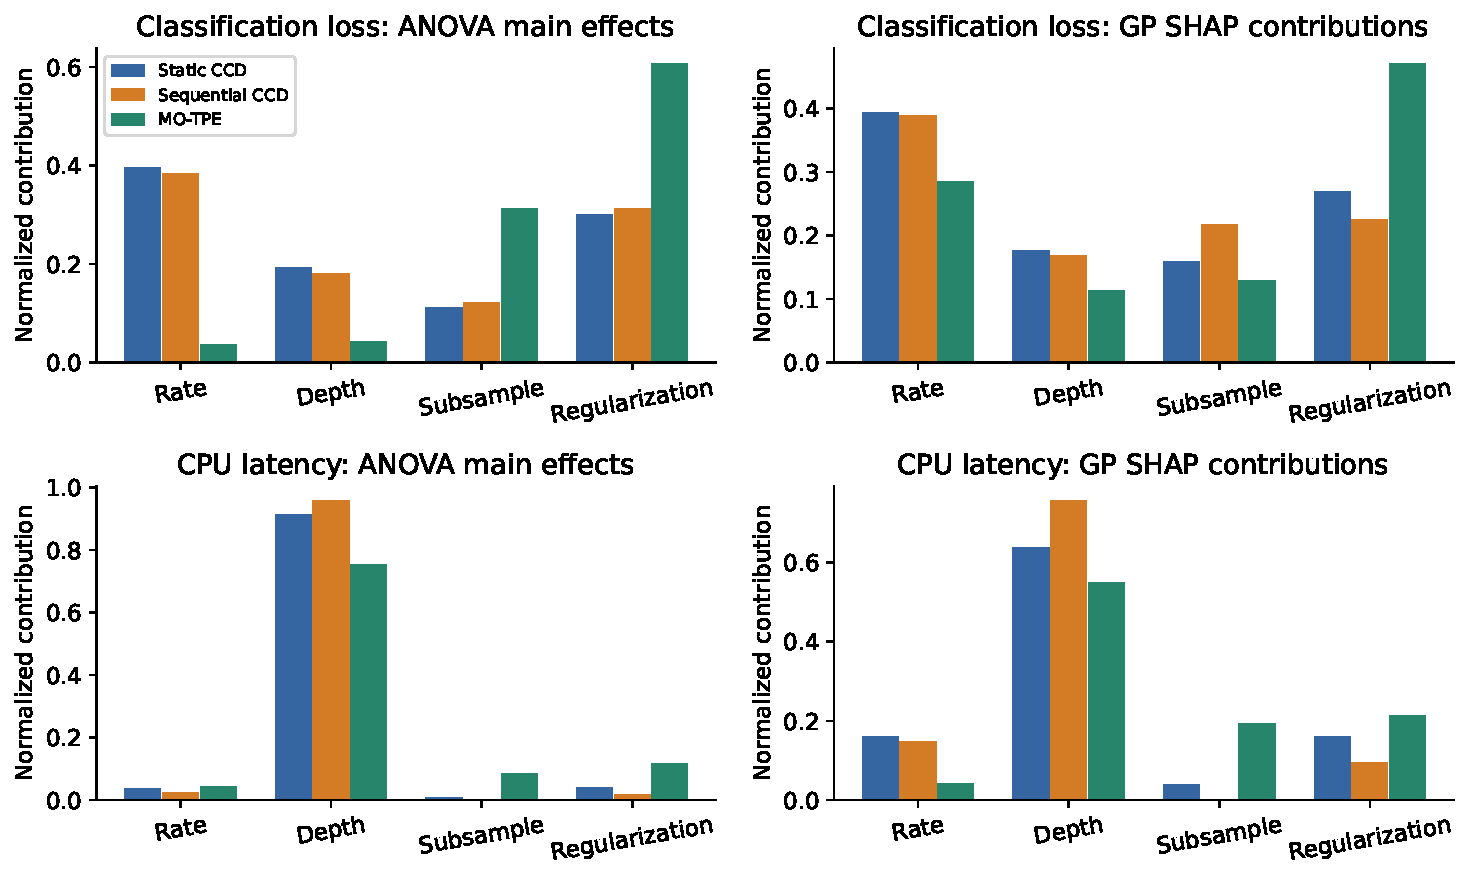
\includegraphics[width=\textwidth]{figures/phase_b_importance.pdf}
\caption{Phase B factor contributions to classification loss and latency. ANOVA main-effect strengths and GP-surrogate SHAP contributions are normalized separately and averaged over repeats. Their relative patterns can be compared; their underlying units and estimands differ.}\end{figure}
\begin{figure}[!htbp]\centering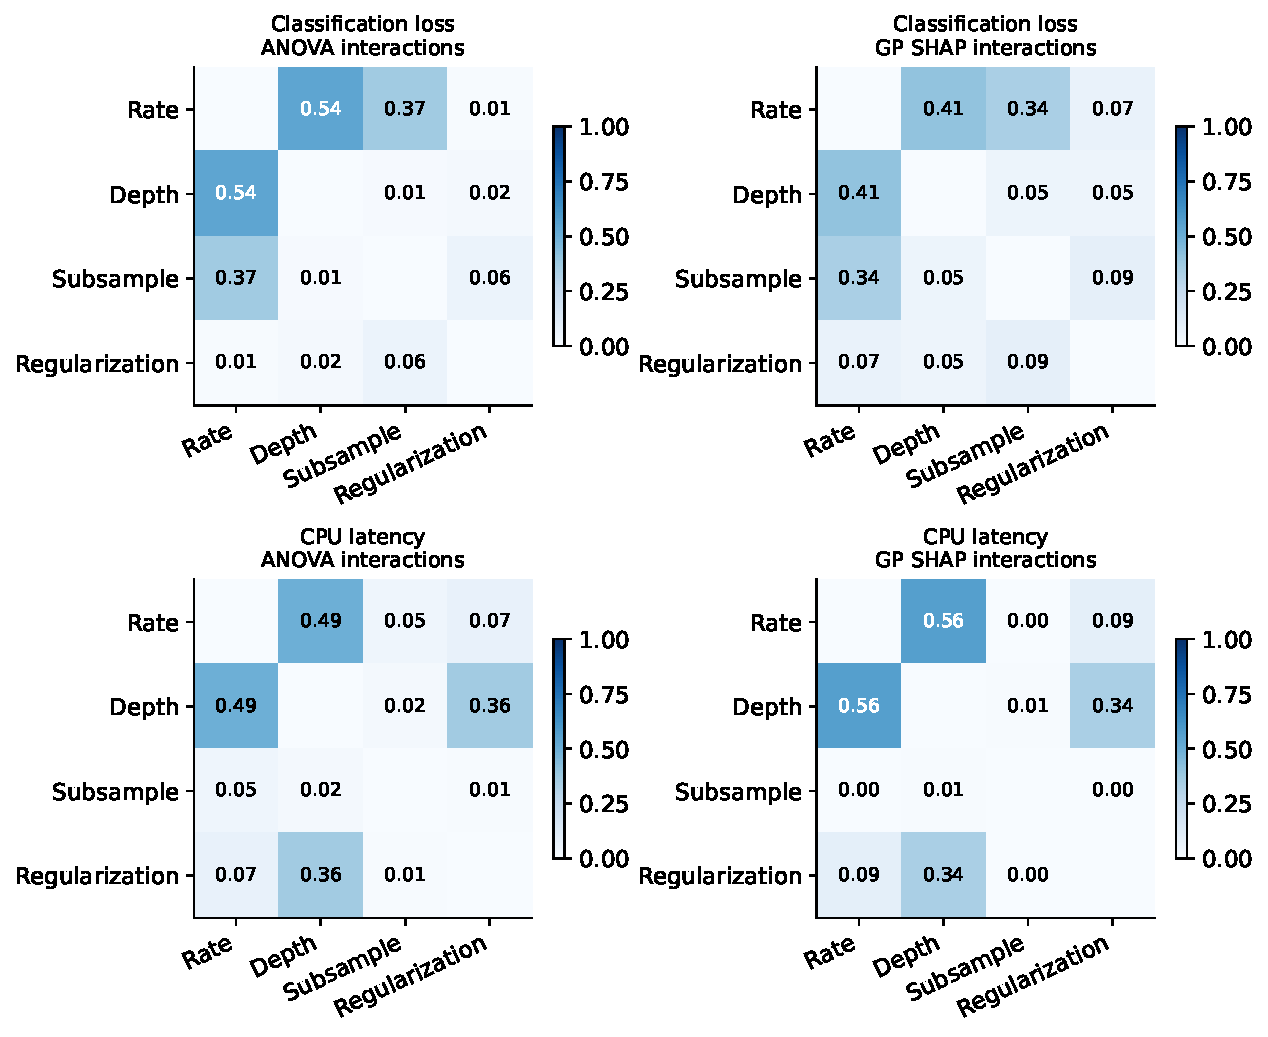
\includegraphics[width=\textwidth]{figures/phase_b_interactions.pdf}
\caption{Pairwise interaction patterns for sequential CCD, averaged over repeats. ANOVA and GP SHAP matrices are normalized independently. Agreement concerns which pairs matter, not numerical equality between variance attribution and Shapley contributions.}\end{figure}
Factor rankings disagree substantively across sampling methods; these data do not identify which attribution is ground truth. High Pearson correlation can also be dominated by the largest pair effects. Table~\ref{tab:leverage} adds pair-rank correlation and an omission check. Both explanation models fit the same observations, so agreement is a consistency diagnostic rather than independent validation.
\begin{table}[!htbp]\centering\small\resizebox{\textwidth}{!}{\begin{tabular}{lrrr}
\toprule
Sampling & Pair-rank correlation & Pearson after omission & Two-pair ANOVA share \\
\midrule
Static CCD & \m{PostLeverageARank} & \m{PostLeverageAOmit} & \m{PostLeverageAShare} \\
Sequential CCD & \m{PostLeverageBRank} & \m{PostLeverageBOmit} & \m{PostLeverageBShare} \\
MO-TPE & \m{PostLeverageCRank} & \m{PostLeverageCOmit} & \m{PostLeverageCShare} \\
\bottomrule
\end{tabular}
}
\caption{Post-hoc interaction checks for classification loss, averaged across repeats. Pair-rank correlation is Spearman correlation over \m{PostPairCount} pairs. The omission column removes the two largest ANOVA interaction pairs within each repeat before recomputing Pearson correlation; the last column gives their combined normalized ANOVA share.}\label{tab:leverage}\end{table}
\begin{figure}[!htbp]\centering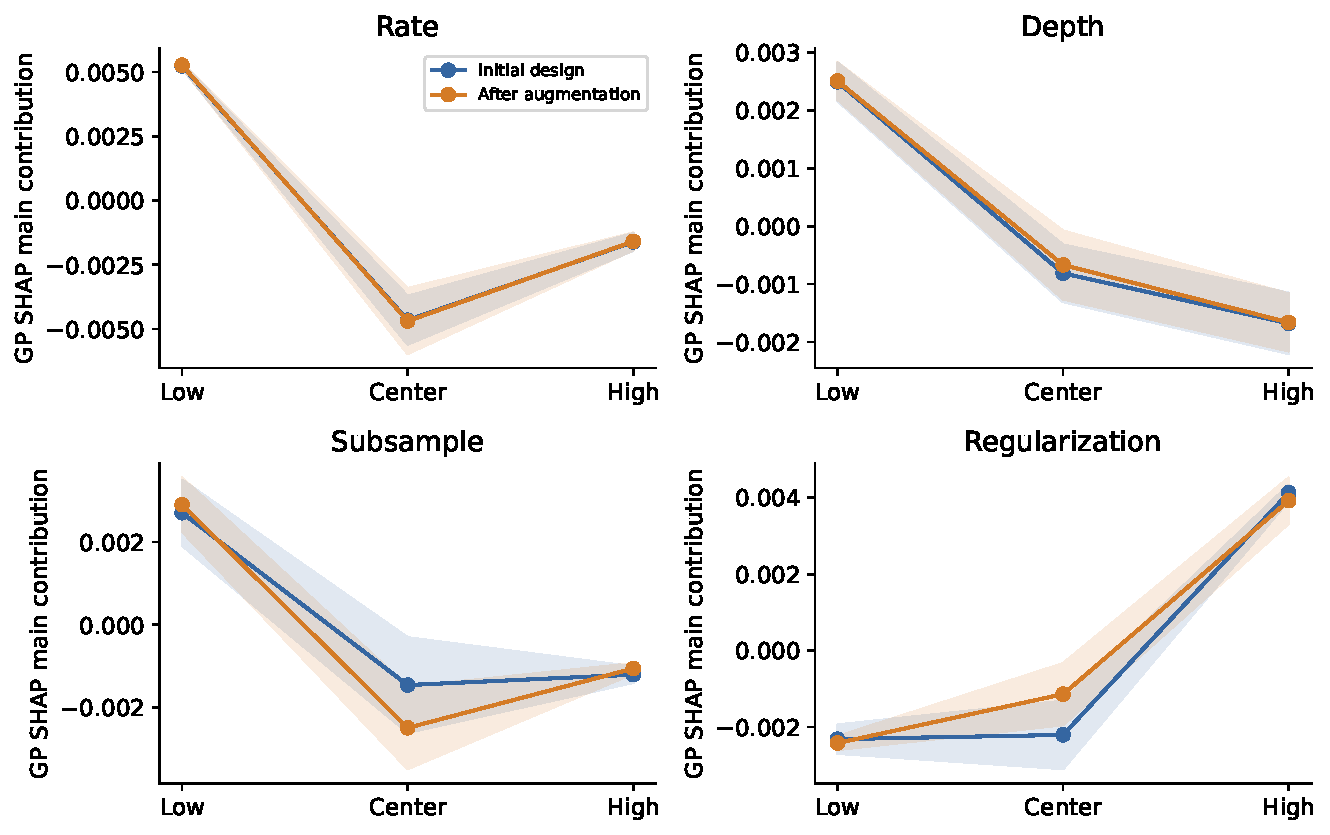
\includegraphics[width=\textwidth]{figures/phase_b_curvature.pdf}
\caption{Nonlinear hyperparameter profiles before and after sequential augmentation. Lines show the mean GP SHAP main-effect contribution at low, center and high settings; bands show variation across search repeats. Curvature is visible as a departure from a straight profile.}\end{figure}
\subsection{New hyperparameter coordinates test response predictions}
The experiment reserves \m{BConfirm} coordinates before search. A fixed seeded generator draws uniformly in coded space, projects depth onto its integer grid and excludes duplicate or initial-design coordinates. Alternating accepted coordinates are additionally assigned to opposite learning-rate faces. Near-boundary values in any factor are tagged using the declared cutoff. Only the coordinates are known during design; their measured responses are excluded from acquisition and surrogate fitting.
\begin{table}[!htbp]\centering\resizebox{\textwidth}{!}{\begin{tabular}{lrrrrr}
\toprule
Method & Response & Pred. RMSE & Mean bias & Coverage & Boundary bias \\
\midrule
Static CCD & Loss & \m{ConfirmAvallossError} & \m{ConfirmAvallossBias} & \m{ConfirmAvallossCoverage}\% & \m{ConfirmAvallossBoundary} \\
Static CCD & Latency & \m{ConfirmAlatencyusError} & \m{ConfirmAlatencyusBias} & \m{ConfirmAlatencyusCoverage}\% & \m{ConfirmAlatencyusBoundary} \\
Sequential CCD & Loss & \m{ConfirmBvallossError} & \m{ConfirmBvallossBias} & \m{ConfirmBvallossCoverage}\% & \m{ConfirmBvallossBoundary} \\
Sequential CCD & Latency & \m{ConfirmBlatencyusError} & \m{ConfirmBlatencyusBias} & \m{ConfirmBlatencyusCoverage}\% & \m{ConfirmBlatencyusBoundary} \\
MO-TPE & Loss & \m{ConfirmCvallossError} & \m{ConfirmCvallossBias} & \m{ConfirmCvallossCoverage}\% & \m{ConfirmCvallossBoundary} \\
MO-TPE & Latency & \m{ConfirmClatencyusError} & \m{ConfirmClatencyusBias} & \m{ConfirmClatencyusCoverage}\% & \m{ConfirmClatencyusBoundary} \\
\bottomrule
\end{tabular}
}
\caption{Post-hoc symmetric confirmation of RSM and GP predictions against the same block-mean target: \m{PostMeanConfirmationN} coordinate-by-repeat outcomes from \m{BConfirm} distinct coordinates. Bias is observed minus predicted; boundary means an absolute coded coordinate reaches \m{BBoundaryCutoff}. Coverage uses nominal \m{BIntervalLevel}\% working intervals. Loss errors are in classification-loss units; latency errors are in microseconds.}\label{tab:bconfirm}\end{table}
This comparison averages the saved fold outcomes before calculating errors for both surrogates. The RSM mean-target interval uses residual variance divided by the fold count plus parameter-estimation variance, assuming independent fold residuals as a working approximation despite overlapping training sets. The GP interval uses its fitted mean-response predictive variance. The targets match while the variance assumptions differ. Low mean-response coverage shows that small prediction errors do not ensure well-calibrated uncertainty.
DOE-sampled surfaces predict the domain-wide reserved coordinates more accurately under both model families. The GP does not remove TPE's loss-prediction disadvantage here. This is evidence about sampling geometry and global response modeling, not proof that DOE is a better optimizer near the promising region where TPE concentrates evaluations.
\begin{figure}[!htbp]\centering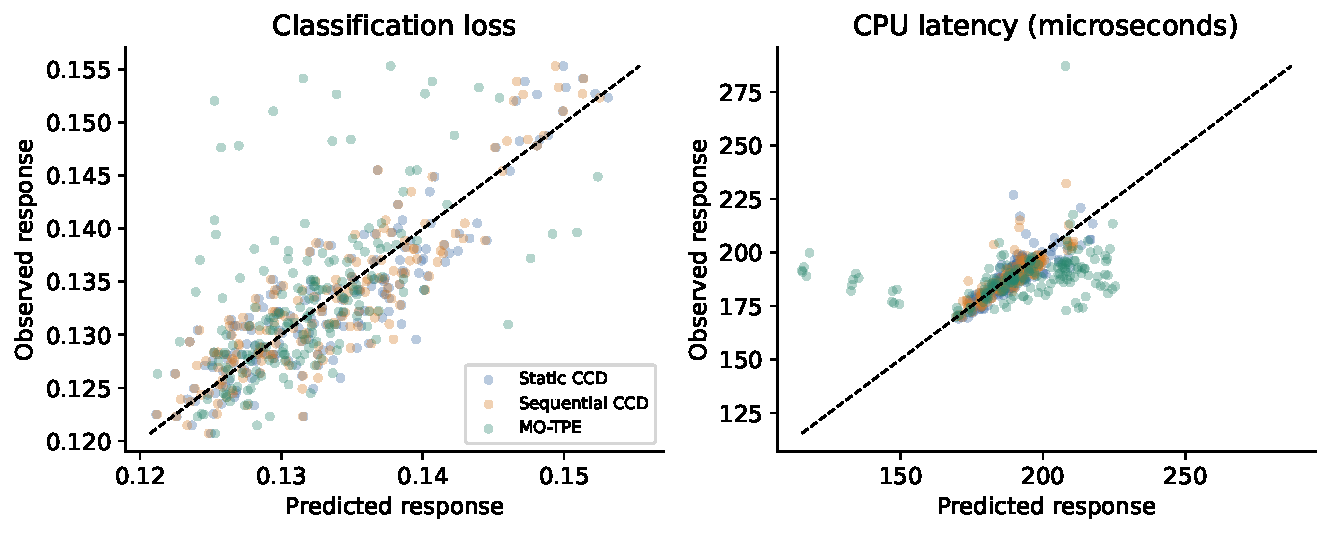
\includegraphics[width=\textwidth]{figures/phase_b_confirmation.pdf}
\caption{Symmetric post-hoc confirmation. Each point compares a predicted coordinate-level mean with its observed mean across the shared folds. RSM and GP use the same reserved outcomes; the dashed line denotes agreement.}\end{figure}
\subsection{Local word explanations answer a separate question}
The word study asks how the probability from one fixed sentiment classifier changes when selected word-feature weights are attenuated. This classifier uses the first sequential-CCD selection, refitted on the training portion of the first development fold; explanations concern that fold's validation documents. A local CCD varies the strongest present unigram features, fits a quadratic probability surface and evaluates fidelity on \m{BWordConfirm} unused perturbations per document. Exact pairwise Shapley values describe the declared feature-weight game.
The study covers \m{BWordDocs} eligible development-validation documents chosen by a fixed label-independent rule. The largest document-level confirmation RMSE is \m{BWordMaxError} probability units. Fidelity varies: some local response functions are simple under these perturbations, while others are less well represented by a quadratic surface.
The original perturbations attenuate selected unigram weights while fixing other features, including bigrams, without renormalization. They describe a conditional feature-weight game rather than rewritten sentences. The illustrated example's maximum recorded endpoint-game pair interaction is \m{PostWordInteractionMax}; zero endpoint interactions do not imply a quadratic continuous probability response. LIME~\cite{lime} and classifier TreeSHAP address related local-explanation questions but were not matched experimental arms, so this study does not establish superiority over either.
\begin{figure}[!htbp]\centering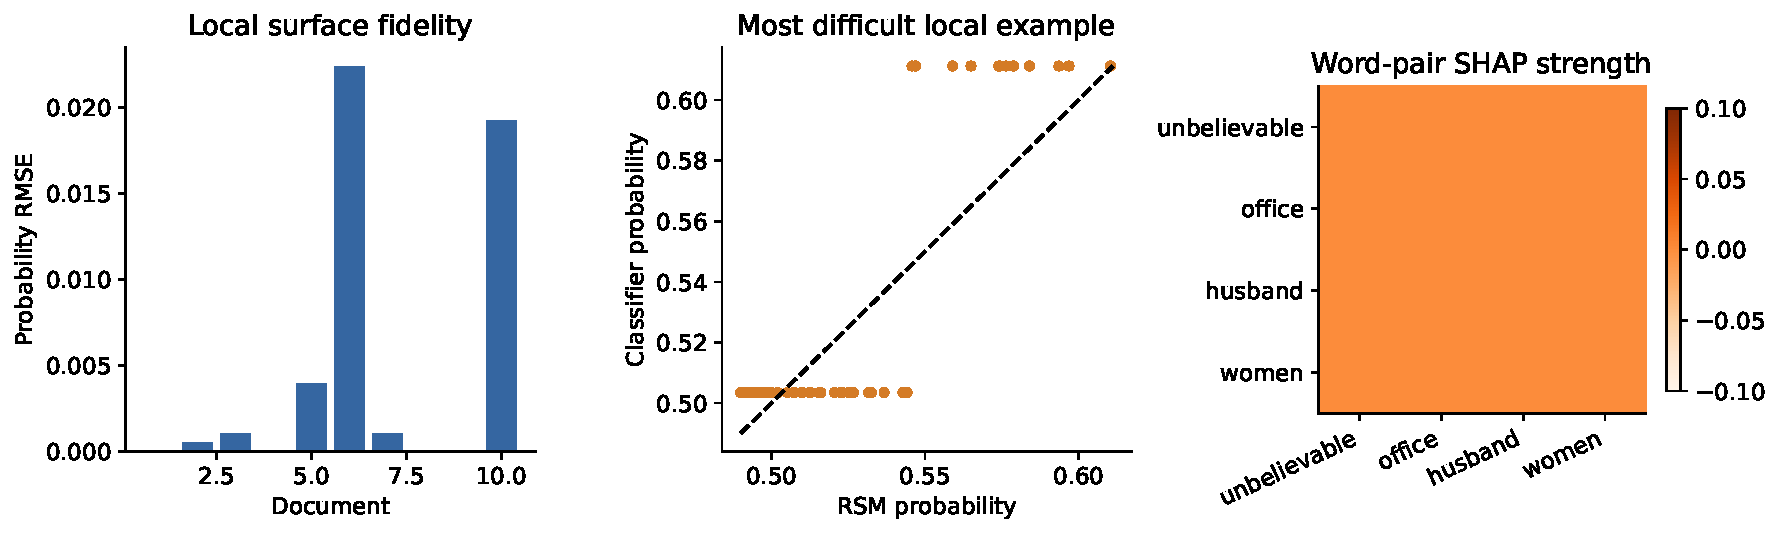
\includegraphics[width=\textwidth]{figures/phase_b_words.pdf}
\caption{Local word responses. Left: fidelity on unused perturbations. Center: the highest-error example, document \m{WordExampleIndex}. Right: signed interactions in its zero/full-retention coalition game, with diagonal masked and all zero pair values annotated. The symmetric color-scale floor is a display choice, not evidence of nonzero interaction.}\end{figure}
\section{Phase B: comparing model quality, latency and adaptation}
\begin{table}[!htbp]\centering\small\resizebox{\textwidth}{!}{\begin{tabular}{lrrrr}
\toprule
Method & Test macro F1 & Log loss & CPU latency ($\mu$s) & Dev. HV \\
\midrule
Static CCD & $\m{BAFone} \pm \m{BAFoneSd}$ & $\m{BALogloss} \pm \m{PostLoglossSdA}$ & $\m{BALatency} \pm \m{PostLatencySdA}$ & $\m{BAHv} \pm \m{BAHvSd}$ \\
Sequential CCD & $\m{BBFone} \pm \m{BBFoneSd}$ & $\m{BBLogloss} \pm \m{PostLoglossSdB}$ & $\m{BBLatency} \pm \m{PostLatencySdB}$ & $\m{BBHv} \pm \m{BBHvSd}$ \\
MO-TPE & $\m{BCFone} \pm \m{BCFoneSd}$ & $\m{BCLogloss} \pm \m{PostLoglossSdC}$ & $\m{BCLatency} \pm \m{PostLatencySdC}$ & $\m{BCHv} \pm \m{BCHvSd}$ \\
\bottomrule
\end{tabular}
}
\caption{Phase B results. Test metrics average the frozen selected classifier from each search repeat. Development hypervolume summarizes each observed search front under its declared reference. The reported dispersions are sample standard deviations across search repeats. Larger F1 and hypervolume are preferable; smaller log loss and latency are preferable.}\label{tab:bbench}\end{table}
Observed test macro F1 is almost the same across methods. The sequential choice has the highest mean in this run, while MO-TPE has the lowest mean selected latency. Static CCD has the highest mean development hypervolume. These small differences do not establish a decisive winner, and absence of a decisive difference does not establish statistical equivalence.
All analyses newly added to the completed campaign are post hoc: paired document bootstrap, capacity-matched comparison, reference sensitivity, transformation diagnostics and interaction omission checks. Table~\ref{tab:bootstrap} uses \m{PostBootstrapCount} paired document resamples~\cite{bootstrap}, applying each resample jointly to all frozen classifiers before averaging within method. Every difference interval includes zero. These intervals quantify document-sampling uncertainty conditional on the trained models; they neither provide more independent optimizer searches nor account for unobserved movie-level clustering.
\begin{table}[!htbp]\centering\small\resizebox{\textwidth}{!}{\begin{tabular}{lrrr}
\toprule
Frozen-model comparison & F1 difference & Lower bound & Upper bound \\
\midrule
Static CCD -- Sequential CCD & \m{PostPairADifference} & \m{PostPairALower} & \m{PostPairAUpper} \\
Static CCD -- MO-TPE & \m{PostPairBDifference} & \m{PostPairBLower} & \m{PostPairBUpper} \\
Sequential CCD -- MO-TPE & \m{PostPairCDifference} & \m{PostPairCLower} & \m{PostPairCUpper} \\
\bottomrule
\end{tabular}
}
\caption{Post-hoc paired bootstrap differences in mean test macro F1, with percentile \m{BIntervalLevel}\% bounds. The same documents are resampled jointly for every frozen classifier. These intervals do not test equivalence or quantify uncertainty over future optimizer runs.}\label{tab:bootstrap}\end{table}
Every frozen selection uses the lower depth boundary, \m{BSelectedDepth}. The reported scores therefore describe shallow compromise models chosen by the common accuracy--latency rule.
No searched block-mean or final selected latency meets the original \m{BCap}\,$\mu$s threshold. Every frozen selection is below the post-hoc capacity-matched reference of \m{PostCapacity}\,$\mu$s. These comparisons use development calibration on different fixed inputs and settings; they are not application-level feasibility guarantees. Table~\ref{tab:operational} retains both comparisons and reports search costs: equal fit budgets did not produce equal elapsed cost. Latency SD across selections is not independent timing-session repeatability, and surrogate prediction error is not an estimate of timing noise.
\begin{table}[!htbp]\centering\small\resizebox{\textwidth}{!}{\begin{tabular}{lrrr}
\toprule
Method & Below original cap & Below matched reference & Search seconds \\
\midrule
Static CCD & \m{PostOperationalAPooled} & \m{PostOperationalAMatched} & $\m{PostOperationalASeconds} \pm \m{PostOperationalASecondsSd}$ \\
Sequential CCD & \m{PostOperationalBPooled} & \m{PostOperationalBMatched} & $\m{PostOperationalBSeconds} \pm \m{PostOperationalBSecondsSd}$ \\
MO-TPE & \m{PostOperationalCPooled} & \m{PostOperationalCMatched} & $\m{PostOperationalCSeconds} \pm \m{PostOperationalCSecondsSd}$ \\
\bottomrule
\end{tabular}
}
\caption{Post-hoc operational comparisons. Counts are out of \m{BRepeats} frozen selections per method. Search seconds are mean $\pm$ sample SD across repeats, including recorded evaluation time and analysis/sampling overhead. Shared preprocessing, calibration, confirmation, final refits and local word analysis are excluded.}\label{tab:operational}\end{table}
The small sequential augmentation does not demonstrate a clear improvement over static CCD. The rectangle score also embeds a preference: at the original loss reference, loss improvement enters through macro F1 while latency enters through distance from its reference. Figure~\ref{fig:sensitivity} varies both reference coordinates on a diagnostic grid, recomputing choices only on existing development observations. Changed choices, including deeper trees, show that the shallow selections are preference-dependent. Newly selected settings are not evaluated on test data, and hypervolume magnitudes under different references cannot be compared directly.
\begin{figure}[H]\centering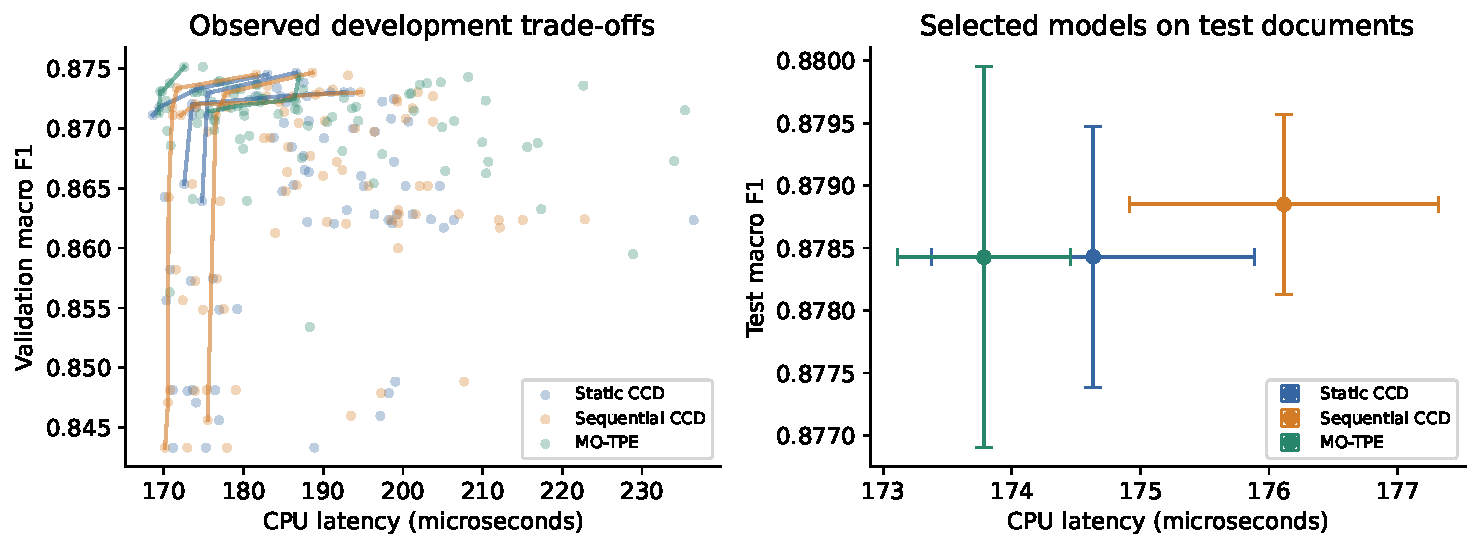
\includegraphics[width=\textwidth]{figures/phase_b_pareto.pdf}
\caption{Phase B accuracy--speed outcomes. Left: observed development configurations and their empirical nondominated fronts for each search repeat. Right: frozen selected models on test documents, with sample standard deviations across search repeats. The right panel evaluates selected points, not a complete test-set search front.}\end{figure}
\begin{figure}[H]\centering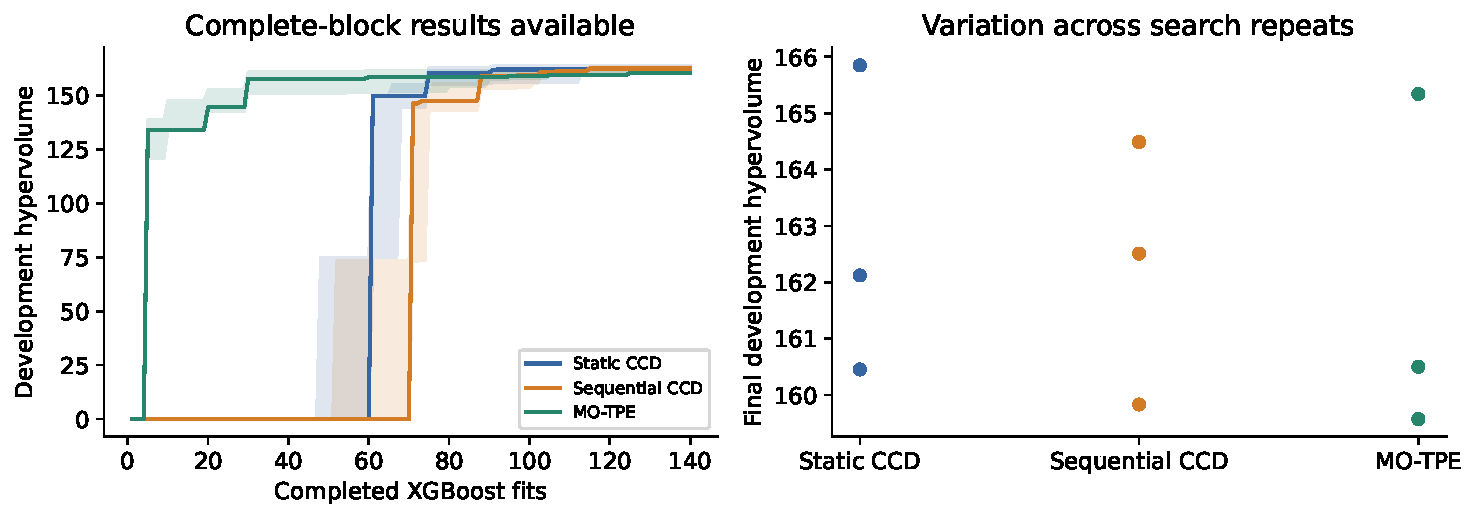
\includegraphics[width=\textwidth]{figures/phase_b_progress.pdf}
\caption{Availability of complete-block Phase B results versus cumulative fits, with final hypervolume variation at right. DOE shuffles evaluations across configurations, while TPE completes each proposal's folds together. DOE's delayed first value therefore reflects scheduling; early curves cannot establish comparative search efficiency. Bands show interquartile ranges. Center-repeat updates can change configuration means.}\end{figure}
\begin{figure}[H]\centering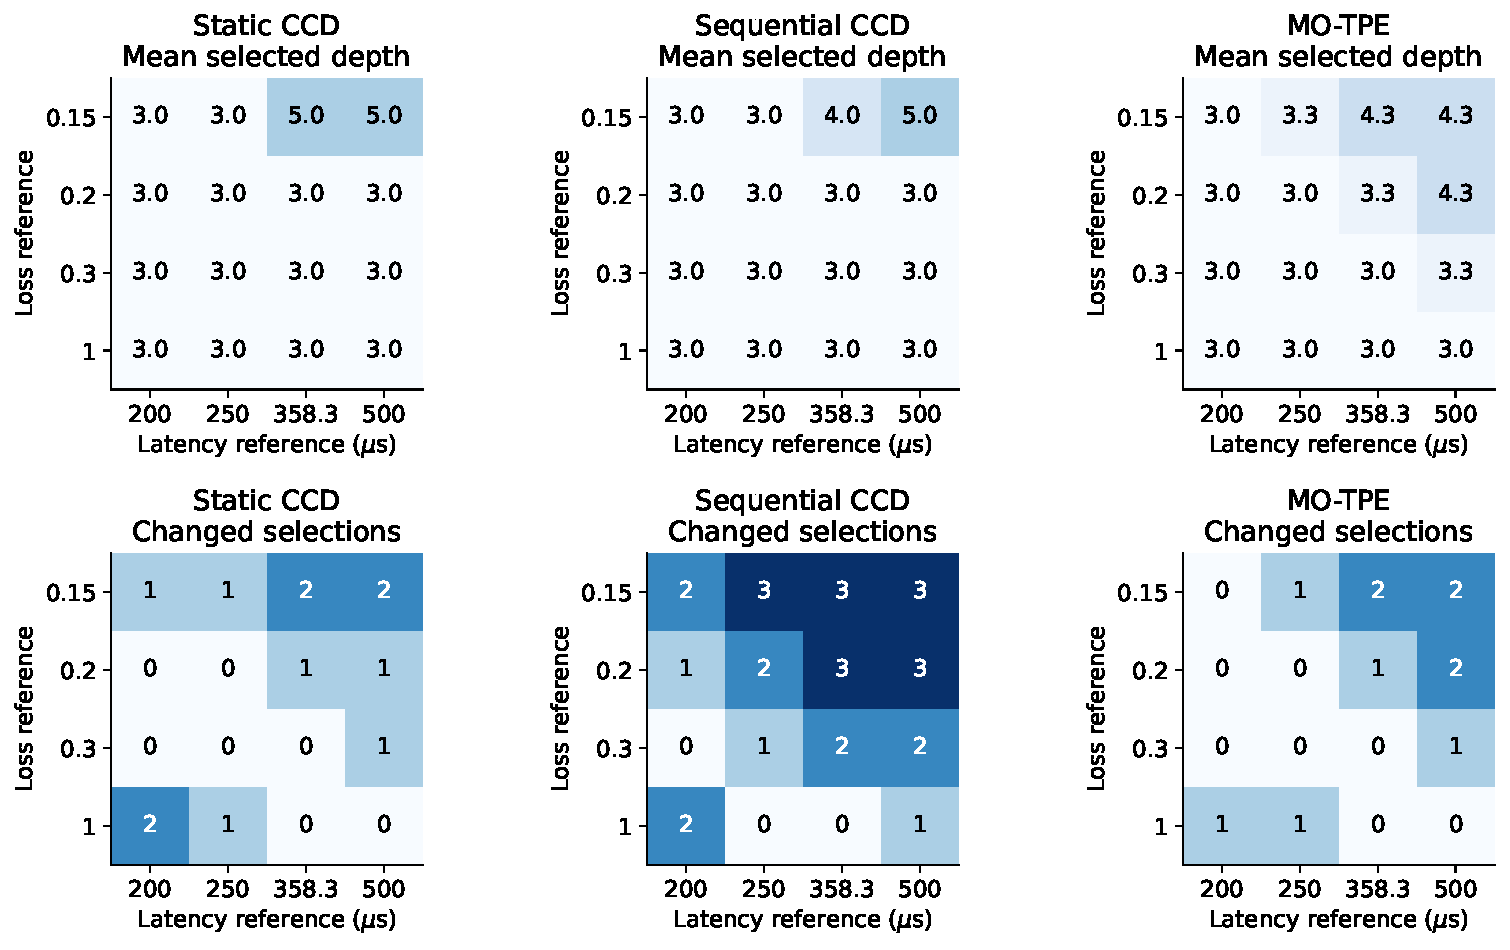
\includegraphics[width=\textwidth]{figures/phase_b_sensitivity.pdf}
\caption{Post-hoc development-only reference sensitivity. Top: mean selected depth across searches. Bottom: selections changed from the original rule, out of \m{BRepeats} per method. Every cell uses the same observed configurations; the grid is not a new search or test-set comparison.}\label{fig:sensitivity}\end{figure}
\section{Discussion}
Phase A shows why optimization and explanation need independent validation. Structured data can reveal curvature and interactions while still producing misleading local predictions. A high-quality fitted summary of a broad domain is not automatically accurate near a selected optimum. Timing precision and historical data exposure also affect what comparisons mean.
Phase B yields similar selected-classifier quality across its sampled methods, with lower recorded search cost for TPE and better domain-wide surrogate prediction from DOE samples. These are distinct outcomes. Diagnostic agreement between fitted explanations helps describe a response model; it does not independently validate the underlying hyperparameter effects. Reference sensitivity and imperfect confirmation coverage further limit what an apparent optimum means.
\subsection{Limitations and threats to validity}
\begin{itemize}
\item \textbf{Replication and information allocation.} Phase B has \m{BRepeats} search repeats and only \m{PostAdaptiveCoordinates} infill coordinates per sequential search. It cannot establish modest method advantages or general conclusions about adaptive design. Phase A compares replicated planned coordinates with broader fixed-split searches. The frozen-model document bootstrap does not resolve either asymmetry. No matched random-search, default-XGBoost or linear-text-classifier arm was included in Phase B.
\item \textbf{Design geometry and explanation.} Face-centered CCD concentrates observations at corners, axial points and repeated centers. Space-filling computer-experiment designs~\cite{sacks,santner} offer a relevant alternative for GP modeling. Global confirmation favors coverage; it is not the same target as finding a good local operating point. Shared-data explanation agreement is not ground truth. The local word study covers \m{BWordDocs} selected documents and a small conditional perturbation game.
\item \textbf{Measurement and inference.} Latency times fresh DMatrix construction and tree traversal on one vectorized input, excluding text vectorization and a representative document distribution. Neither a fitted intercept nor surrogate RMSE isolates system overhead or repeatability. Thresholds and reference points encode calibration and preference choices. Overlapping folds invalidate treating all fold outcomes as independent dataset replications; nominal working-model intervals require empirical checking.
\item \textbf{External validity and evaluation history.} Both test partitions had been evaluated in earlier exploratory work. Freezing selections before this campaign's test access ensures within-run separation but does not restore untouched external confirmation. IMDb folds are stratified by sentiment rather than grouped by movie; movie-level metadata was unavailable to this protocol. The two tasks cannot establish broad applicability, and GPU refits are not guaranteed bitwise reproduction.
\end{itemize}
\subsection{Methodology for a new replication}
The direct Phase B runner now provides opt-in capacity-matched calibration, text-length-stratified timing panels and coupled, normalized TF-IDF perturbations. Their default settings reproduce the historical procedure, and their new protocols are recorded before evaluation. No results from these alternatives are presented as findings of the completed campaign. A stronger comparison still requires matched baseline arms, a larger adaptive allocation, search replication chosen for a predeclared meaningful effect, comparable wall-clock budgets and an independently controlled test dataset. A future SHAP-driven acquisition arm must actually use attribution information in its decision rule.
\section{Conclusion}
Planned experiments provide observations that support both model selection and interpretable response modeling. Phase A demonstrates why broad structure is insufficient to guarantee local predictive adequacy. Phase B distinguishes GP-guided sampling, observed-point selection and diagnostic explanations: selected F1 scores are similar, DOE sampling supports better global response prediction, and the small sequential augmentation yields no established advantage. Post-hoc bootstrap, timing and preference analyses sharpen the interpretation without creating new independent experiments. The contribution is a transparent empirical framework for comparing these roles; efficiency gains, explanation correctness and external generalization remain questions for a stronger replication.
\section{Data and code availability}
The manuscript, prepared data, frozen observations and analysis code are available at \url{https://github.com/ChristosHussein/xgboost-doe-rsm}. The original campaign remains unchanged; the new diagnostics are explicitly post hoc. Appendix~\ref{app:execution} gives commands for saved-result reconstruction and separate CPU or CUDA replications, including the opt-in protocol extensions.
\addcontentsline{toc}{section}{References}
\begin{thebibliography}{9}\small
\bibitem{xgboost} T. Chen and C. Guestrin. \emph{XGBoost: A Scalable Tree Boosting System}. KDD, 2016. \url{https://doi.org/10.1145/2939672.2939785}.
\bibitem{ccd} NIST/SEMATECH. \emph{e-Handbook of Statistical Methods: Central Composite Designs}. \url{https://www.itl.nist.gov/div898/handbook/pri/section3/pri3361.htm}.
\bibitem{housing} Scikit-learn developers. \emph{California Housing dataset}, dataset documentation. \url{https://scikit-learn.org/stable/datasets/real_world.html#california-housing-dataset}.
\bibitem{tpe} J. Bergstra, R. Bardenet, Y. Bengio and B. K\'egl. \emph{Algorithms for Hyper-Parameter Optimization}. Advances in Neural Information Processing Systems, 2011. \url{https://papers.nips.cc/paper/4443-algorithms-for-hyper-parameter-optimization}.
\bibitem{optuna} T. Akiba, S. Sano, T. Yanase, T. Ohta and M. Koyama. \emph{Optuna: A Next-generation Hyperparameter Optimization Framework}. KDD, 2019. \url{https://arxiv.org/abs/1907.10902}.
\bibitem{shap} S. M. Lundberg and S.-I. Lee. \emph{A Unified Approach to Interpreting Model Predictions}. Advances in Neural Information Processing Systems, 2017. \url{https://arxiv.org/abs/1705.07874}.
\bibitem{interactions} S. M. Lundberg, G. G. Erion and S.-I. Lee. \emph{Consistent Individualized Feature Attribution for Tree Ensembles}. arXiv, 2018. \url{https://arxiv.org/abs/1802.03888}.
\bibitem{imdb} A. L. Maas, R. E. Daly, P. T. Pham, D. Huang, A. Y. Ng and C. Potts. \emph{Learning Word Vectors for Sentiment Analysis}. ACL, 2011. \url{https://aclanthology.org/P11-1015/}.
\end{thebibliography}

\clearpage
\appendix
\section{Reproducibility and execution commands}\label{app:execution}
\subsection{Obtain the repository and install the environment}
The code, manuscript and lossless saved-result archive are available at \url{https://github.com/ChristosHussein/xgboost-doe-rsm}. The fixed tag \texttt{paper-2026-10-r3} identifies this paper's revision. The following PowerShell commands use the repository root and the pinned reference environment:
\begin{lstlisting}
git clone https://github.com/ChristosHussein/xgboost-doe-rsm.git
cd xgboost-doe-rsm
git checkout paper-2026-10-r3
python -m venv .venv
.\.venv\Scripts\Activate.ps1
python -m pip install -r requirements-reproduction.txt
python report/restore_evidence.py
python report/verify_report.py --check
\end{lstlisting}
These commands check the saved results without training new classifiers. The compressed observations are in \texttt{evidence/phase\_b.zip}; restoration preserves their original bytes and refuses to overwrite different local results. Phase A observations are stored under \texttt{phase\_a\_rsm\_blocking/results}. The reference measurement contracts record source hashes, dependencies and hardware. A new training run is an experimental replication whose timings may differ.
\subsection{Start with the smoke verification}
\begin{lstlisting}
python run_experiment.py --smoke
\end{lstlisting}
This performs a small synthetic execution check before a full experiment; it does not add scientific observations to the reported campaign.
\subsection{Run Phase A on CPU}
The master command runs the revised repeated benchmark rather than silently overwriting the historical housing design:
\begin{lstlisting}
python run_experiment.py --phase a --mode full
\end{lstlisting}
For explicit output control, the direct runner supports a fresh destination and budget acknowledgement:
\begin{lstlisting}
python phase_a_rsm_blocking/scripts/run_benchmarks.py --mode full --confirm-full-budget --output-dir results/housing_new_run
\end{lstlisting}
The Phase A runner supports \texttt{--resume} for interrupted checkpointed runs. Phase A uses CPU training. The historical response-surface study and repeated benchmark are separate experiments.
\subsection{Run Phase B with CUDA training or CPU training}
For a new CUDA campaign, use the direct Phase B runner so output and calibration paths are explicit:
\begin{lstlisting}
python phase_b_sequential_xai/run_phase_b.py --stage all --dataset full_imdb --data-dir phase_b_sequential_xai/data --calibration-dir results/imdb_cuda_new/calibration --output-dir results/imdb_cuda_new --findings-dir findings/imdb_cuda_new --device cuda
\end{lstlisting}
For CPU-only training, change the device and use a separate output destination:
\begin{lstlisting}
python phase_b_sequential_xai/run_phase_b.py --stage all --dataset full_imdb --data-dir phase_b_sequential_xai/data --calibration-dir results/imdb_cpu_new/calibration --output-dir results/imdb_cpu_new --findings-dir findings/imdb_cpu_new --device cpu
\end{lstlisting}
CUDA training requires a CUDA-enabled XGBoost installation and compatible NVIDIA hardware and driver. The measured run records an \AcceleratorName{}; other compatible hardware can run the method but may produce different timings. CUDA accelerates classifier training; surrogate analysis and the prediction-latency operation remain on CPU.
The \texttt{--training-threads} option controls training-side CPU workers; it does not change the frozen single-thread inference measurement. \texttt{--device auto} selects a device automatically. An explicit \texttt{cuda} or \texttt{cpu} setting makes the computational configuration reproducible.
\subsection{Opt-in protocols for a new replication}
The direct Phase B runner additionally supports the following options; the root master command does not forward these flags:
\begin{lstlisting}
--threshold-mode capacity_matched
--latency-panel-size 32
--consistent-tfidf-perturbations
\end{lstlisting}
The panel-size example is an execution setting rather than a reported measurement. Defaults remain \texttt{pooled}, a single timing document, and uncoupled unnormalized perturbations. Capacity matching takes the median across all calibration records at the selected capacity. Multi-document timing chooses a label-free character-length-stratified panel within each fold and cycles fresh single-row DMatrix calls over it; final panel construction remains behind the frozen-selection gate. Calibration and main-run panel protocols must match.
The coupled word option multiplies active bigram weights by the attenuations of their selected constituent tokens and then normalizes the sparse vector. It still defines a feature-space game, not a grammatical edit or causal intervention. Supplemental contracts record these options and extension source hashes before evaluation; new outputs must use a fresh directory. These protocols have synthetic execution checks but no new real-data results in this paper.
\subsection{Run individual stages and verify saved evidence}
The stages \texttt{prepare}, \texttt{calibrate}, \texttt{run} and \texttt{generate-findings} can be executed separately. The \texttt{run} stage includes the local word study; \texttt{all} runs the complete pipeline. Use a fresh output directory for each replication. Phase B does not provide checkpoint resumption.
To verify a completed Phase B study without retraining:
\begin{lstlisting}
python phase_b_sequential_xai/run_phase_b.py --check results/phase_b/imdb
\end{lstlisting}
To regenerate only its findings, with the raw evidence available:
\begin{lstlisting}
python phase_b_sequential_xai/run_phase_b.py --stage generate-findings --dataset full_imdb --output-dir results/phase_b --findings-dir findings/reconstructed_imdb
\end{lstlisting}
The alternative \texttt{yelp} dataset option supports a separate sentiment application. The Phase B results reported here concern IMDb.
To rebuild the paper's tables and figures from the published observations, run \texttt{python report/build\_evidence.py}, then compile \texttt{report/report.tex} with pdfLaTeX from its directory. Recalibration on another machine defines a new replication whose timing results should be reported separately.
\end{document}
